\documentclass[12pt]{article}
\usepackage[utf8]{inputenc}
\usepackage[english]{babel}
\usepackage{csquotes} % 
\usepackage{url}
\usepackage[hyperfootnotes=false]{hyperref}
\usepackage[backend=biber, natbib=true, style=authoryear, giveninits=true, citestyle=apa, maxcitenames=2, maxbibnames=99, sorting=nyt, dashed=false]{biblatex}
\renewbibmacro{in:}{}
\renewbibmacro*{doi+eprint+url}{%
  \iftoggle{bbx:doi}
    {\iffieldundef{doi}{}{% 
       \newunit\newblock
       \printtext{%
         \url{https://doi.org/\thefield{doi}}% 
       }%
     }%
    }%
    {}%
  \newunit\newblock
  \usebibmacro{finentry}% Finalizes the entry
}
\addbibresource{export.bib}

\usepackage{graphicx} % Required for inserting images
\usepackage{setspace}
\usepackage{rotating}
\usepackage{tabularx}
\usepackage{booktabs}
\usepackage{amsmath}
\usepackage{csquotes}
\usepackage[usenames,dvipsnames]{color}
\hypersetup{
  colorlinks,
  citecolor=black,
  linkcolor=black,
  hypertexnames=true,
  urlcolor=blue}
\usepackage{appendix}
\doublespacing
\usepackage{float}
\usepackage{titlesec}
\setlength{\headheight}{14.49998pt}
\titleformat{\section}
  {\normalfont\normalsize\bfseries}{\thesection}{1em}{}
\titleformat{\subsection}
  {\normalfont\normalsize\bfseries}{\thesubsection}{1em}{}
\titleformat{\subsubsection}
  {\normalfont\normalsize\bfseries}{\thesubsubsection}{1em}{}
\usepackage{derivative}
\usepackage{fancyhdr}
\usepackage{geometry}
\geometry{
 a4paper,
 total={15cm,22cm},
 top=3.85cm,
 bottom=3.85cm,
 }
 \setstretch{1.83}
 \usepackage[tracking=alltext,letterspace=90]{microtype}
\microtypesetup{protrusion=true, expansion=true}
\usepackage{ragged2e}
\pagestyle{fancy}
\fancyhf{} 
\fancyhead[R]{\thepage}  
\renewcommand{\headrulewidth}{0pt}  
\usepackage{footmisc} 
\setlength{\footnotesep}{1em}  
\renewcommand{\footnotelayout}{\setstretch{1.5}}  

\begin{document}
\begin{titlepage}
    \begin{center}
        \doublespacing 
        \vspace*{1in} 
        {\Large \bfseries Heterogeneity and Non-Linearities in International R\&D Spillovers: Evidence from 23 OECD Countries}\\[1.5cm]
        {\Large Shreesh Chary}\\[0.5cm]
        {\large School of Economics, University of Nottingham, United Kingdom, NG7 2RD} \\[2cm]
        \textit{This dissertation is presented in part fulfilment of the requirement for the completion of an MSc in the School of Economics, University of Nottingham.  The work is the sole responsibility of the candidate.}\\[2cm]
        Submission Date: 19 September 2024\\[0.5cm]
        Supervisor: Professor Facundo Albornoz Crespo\\[0.5cm]
        Word Count: 7040 \\[2cm]
    \end{center}
\end{titlepage}

\newpage
\setcounter{page}{2}
\begin{abstract}
This study explores the influence of international knowledge spillovers on productivity across 23 OECD countries over 49 years, focusing on the role of economic size, human capital, and import intensity. Using a dynamic Common Correlated Effects (CCE) estimator, it addresses cross-sectional dependency and unobserved common shocks that may bias traditional estimates. The findings challenge previous studies by showing statistically insignificant long-run effects of both domestic and foreign R\&D stocks. The results reveal that G7 countries and countries with higher levels of human capital gain more from domestic R\&D, while the benefits of foreign R\&D diminish as import intensity increases. Additionally, non-linear relationships between foreign R\&D and productivity are observed in countries with lower import share of GDP.  \\
\textit{\textbf{Keywords:} Dynamic CCE, Economic Growth, Productivity, R\&D, Spillovers}\\
\textit{\textbf{JEL Classification}: O31, O33, O40}
\end{abstract}

\newpage
\tableofcontents

\newpage

\section{Introduction}

Economic growth has always been a central concern for economists and policymakers around the world. Since the industrial revolution, economic growth has allowed people to afford a lifestyle that only a few ultra-rich people could afford before \citep{Aghion1998}. Building on the seminal work of \citet{Solow1956}, which identified technical progress as the primary driver of such economic growth, endogenous growth models have argued that incentivised innovation in the form of research and development\footnote{This paper focuses solely on R\&D by the business sector} (R\&D) investments, drives technical progress, enhancing productivity\footnote{Productivity and total factor productivity (TFP) have been used interchangeably throughout this study} growth across countries. This innovation can be thought of in two ways: the first being an innovation in the number of inputs, or ``horizontal” innovation, as illustrated by \citet{Romer1990}; the second is an innovation in the quality of inputs, where each innovation leads to knowledge creation on a technological frontier \citep{Grossman1991ql, Aghion1992}. These innovation efforts explain why countries experience varying stages of economic growth based on the extent of their R\&D activities.

Although growth models show that a country's R\&D efforts determines its productivity, countries do not rely solely on their domestic firms for production inputs; they also import inputs from abroad. Due to access to foreign markets through trade, domestic productivity depends on both domestic and foreign R\&D efforts \citep{Grossman1991}. This viewpoint motivates the possibility of R\&D spillovers\footnote{R\&D spillovers and knowledge spillovers have been used synonymously throughout this paper}: R\&D effort undertaken by one country influences the productivity of another. The rationale behind the use of the phrase ``spillover" is that R\&D is a non-rival good; the marginal cost of an additional firm or individual using a technology is negligible \citep{Keller2004, Romer1990}. Hence, the benefits of innovation are not reaped by the innovating country alone, but also by the importing economy. 
	 
The seminal empirical work by \citet{Coe1995} demonstrates that both domestic and foreign R\&D stocks significantly influence a country's productivity. However, much of the subsequent cross-country studies on international R\&D spillovers (most recent of which is the study by \citet{Coe2009}) have relied on methods that assume cross-sectional independence of errors, overlooking the potential for unobserved common shocks and spillovers to cause contemporaneous correlations (cross-sectional dependency) across countries. Recent panel time-series literature\footnote{See \citet{Chudik2015} for a more comprehensive review} has progressed by adopting techniques that are robust to cross-sectional dependency, rendering previously used methods in the international R\&D spillovers literature outdated. Furthermore, a recurring finding in the literature is that greater trade openness, typically measured by the import share of GDP, leads to higher R\&D spillovers \citep{Coe1995, Coe2009, Lichtenberg1998}. However, the validity of this conclusion is questionable: does it imply that countries should indiscriminately increase their imports to boost domestic productivity? It is possible that previous studies have mischaracterised the role of trade openness as a mediator in influencing R\&D spillovers.

Using data from 23 OECD countries from 1971 to 2019, this study employs a dynamic common correlated effects (CCE) estimator to address two research objectives. First, it seeks to investigate international R\&D spillovers by capturing unobserved common shocks that previous studies have overlooked. The results show that while traditional methods assuming cross-sectional independence produce findings consistent with existing literature, the CCE estimator reveals that the impact of foreign R\&D stocks on productivity is insignificant. Second, the study empirically tests for non-linearities in international R\&D spillovers. It finds evidence of such non-linearities in countries where the average import intensity is below 15\%, showing that spillover effects initially rise and eventually fall as import intensity rises. 

The remainder of this paper is organised as follows: Section 2 establishes the theoretical framework. Section 3 describes the construction of variables and presents summary statistics. Section 4 elaborates on the methodology used in the paper. Section 5 presents the results of the econometric model and discusses its implications on the broader growth literature. Section 6 concludes.

\section{Theoretical Framework}

The literature on international R\&D spillovers has developed around two main themes. First, theoretical models and empirical studies highlight the significant impact of incentivised R\&D activities on productivity growth. For example, \citet{Grossman1991} points out that trade openness enhances productivity by enabling R\&D spillovers through the importation of high-quality inputs. \citet{Dixit1977} argue that increasing the variety of available inputs improves total factor productivity, as new inputs contribute to the overall stock of knowledge and reduce future R\&D costs. Through trade, these spillovers can transcend national borders, implying that R\&D activities in one country can influence the R\&D expenditures and productivity of another \citep{Coe2009}. The degree to which foreign countries benefit from these spillovers may be affected by factors such as the volume of bilateral trade between countries or the nature of the traded products.

\citet{Coe1995} investigate the theory established by \citet{Grossman1991} for 22 OECD countries using bilateral import weights for foreign R\&D stocks and find that both domestic and foreign R\&D stocks successfully explain more than half of the variation in TFP between 1971 and 1990. However, \citet{Lichtenberg1998} state that the bilateral import weights method suffers from aggregation and indexation issues. They construct a weighing scheme where weights are chosen based on the ratio of bilateral imports to the exporting partner's nominal GDP. However, they arrive at results that are very similar to \citet{Coe1995} and show that countries that are more open to trade experience greater R\&D spillovers. Furthermore, recent evidence by \citet{Fracasso2015} show that trade patterns significantly affect international R\&D spillovers. In summary, import intensity, trade openness, and trade patterns are key determinants of international R\&D spillovers.

Secondly, there is a methodological debate on how to measure domestic R\&D stocks, as R\&D is inherently difficult to quantify. Common approaches include evaluating inputs, such as R\&D expenditures, and outputs, such as patents. While the OECD provides internationally comparable R\&D data, this data largely represents wealthier countries, often excluding poorer nations that focus more on technology adoption than innovation \citep{Keller2010}. Most empirical studies have relied on business sector R\&D stocks constructed via the perpetual inventory method using OECD R\&D expenditure data \citep{Coe1995, Coe1997, Coe2009, Engelbrecht1997}. Alternatively, patents provide another method of constructing R\&D stocks, potentially offering broader inclusivity. \citet{Madsen2007} uses a panel of 16 OECD nations over 135 years, finding that both domestic and foreign R\&D stocks, constructed from patent data, significantly influence productivity growth. Similarly, \citet{Lee2006} investigates the effectiveness of different spillover channels, including FDI and imports, using patent data, and concludes that while the import of intermediate goods is not an effective channel for international R\&D spillovers, FDI emerges as the most potent one. However, using patent data to analyze spillovers has its drawbacks. Patents can be misleading since a small number of patents account for most of the value, not all innovations are patented, and non-codifiable technologies are excluded \citep{Jaffe2002}. 

\subsection{Sources of Heterogeneity in Spillovers}

This study explores two sources of heterogeneity. First, larger countries\footnote{``Large countries" refers to economic size rather than geographic size} typically engage in a wide array of R\&D activities, which allows them to better leverage complementarities across different sectors, resulting in higher returns on their domestic R\&D investments \citep{Coe1995}. As a result, it is expected that the coefficients for domestic R\&D stocks will be higher for large countries, reflecting their ability to capitalize on these synergies and promote economic growth. In contrast, smaller countries often lack the scale and scope to develop their own cutting-edge technologies, leading them to focus more on adopting foreign technologies \citep{Santacreu2015}. This reliance on external innovation suggests that non-G7 countries would typically exhibit a larger coefficient for foreign R\&D stocks.  

Second, human capital also plays a crucial role in shaping a country's ability to absorb foreign R\&D \citep{Nelson1966}. Theoretically, human capital influences spillovers in two ways. First, vintage human capital models, as discussed by \citet{Chari1991}, suggest that countries with limited R\&D spillovers may be characterised by specialised technology expertise, or ``vintage human capital." \citet{Jovanovic1996} state that such specialized knowledge can reduce the incentive to adopt new technologies, as switching might mean losing the benefits of accumulated expertise. Consequently, both workers and firms may continue investing in older technologies despite the availability of newer, potentially superior alternatives. On the other extreme, firms might be compelled to adapt, leading to increased productivity and potentially positioning these countries as ``early adopters" of new technologies \citep{Barro1997}. These two possibilities highlight the role of human capital in a country's ability to absorb foreign R\&D. 

\citet{Coe1997} revisit the \citet{Coe1995} model by incorporating educational attainment as an indicator of human capital. Similarly, \citet{Engelbrecht1997} utilizes data on average years of schooling from \citet{Barro2001} to examine the impact of human capital. Both studies find that human capital positively and significantly affects the elasticity of both domestic and foreign R\&D stocks. Furthermore, \citet{Coe2009} builds on this by demonstrating that human capital contributes to cross-country heterogeneity, with countries possessing greater human capital showing higher elasticities for domestic and foreign R\&D stocks. Hence, this study controls for human capital and analyses parameter heterogeneity based on differences in human capital. 

\subsection{Non-Linearities in R\&D Spillovers}

Since the the main channel of R\&D spillovers explored in this study is imports, it is also important to acknowledge that import competition, which is directly linked with trade openness \citep{Chen2009}, may have a mediating negative effect on R\&D spillovers. To that end, there are two contrasting, yet plausible outcomes of increased import competition: one, it may retard productivity growth by reducing profitability of domestic innovation \citep{Autor2020, Feenstra1996}; and two, import competition may be productivity enhancing, by incentivising domestic firms to ramp up their innovation to meet import competition \citep{Baldwin1992, Bloom2016}. Furthermore, \citet{Aghion2005} theorise that competition from imports drives productivity growth and increases R\&D spending among domestic firms and industries that are closer to the global technological frontier. However, for firms and industries that are trailing behind, such competitive pressure tends to reduce their motivation to invest in productivity enhancements and R\&D. Evidence suggests that there may, therefore, be an inverted U-shaped non-linear relationship between import competition and productivity growth \citep{Aghion2005}. In this context, \citet{Acharya2008} observe that while import liberalization can reduce domestic productivity over the long term, it can also foster technological learning, especially when imports are technology-intensive. 


The nature of the above non-linearities\footnote{I label this effect as a non-linearity rather than heterogeneity because the weighing scheme for foreign R\&D depends on imports; higher imports result in a higher stock of foreign R\&D. Hence, the relationship between productivity and foreign R\&D is understood to be non-linear in imports.} can be theoretically justified using existing literature. As imports rise, the influx of foreign goods increases competitive pressure on domestic firms, potentially leading to market distortions and productivity losses. The justification for the effect of R\&D stocks on TFP being a decreasing function in imports can be attributed to two relationships specified by \citet{Aghion2005}. They theorise that in a low-competition environment, a greater proportion of sectors tend to feature incumbents that are closely matched, making it more probable that an ``escape-competition" effect will prevail, suggesting that firms innovate to avoid losing market share to close competitors. Conversely, in a high-competition context, the ``Schumpeterian" effect is more likely to take precedence because a larger number of sectors are characterised by lagging firms with initially low profits taking the lead in innovation. Here, the Schumpeterian effect emphasises that intense competition encourages less profitable firms to innovate as a means to catch up or survive in the market. Hence, this study hypothesises that spillovers initially rise with import intensity, but eventually peaks and starts falling as import intensity continues to increase.

\subsection{Unobserved Common Shocks and Spillovers}

Technology has become global as it has been made available to individuals worldwide through new telecommunications and internet technologies and growing economic interconnectedness \citep{Keller2010}. Foreign knowledge that disseminates through a particular channel and remains unobserved may blend with R\&D spillovers transmitted through other channels, such as FDI, patent flows, imports and exports, and geographic proximity \citep{Lee2006, Keller2010}. These channels of international R\&D spillovers may be unobserved in the specifications tested, but strongly influence the estimates of the growth regressions, and therefore should not be ignored \citep{Eberhardt2013}. Furthermore, unobserved common shocks may also influence factors such as freight and insurance, trade costs, and international political relations. For instance, \citet{Moretti2023} show that an increase in military R\&D expenditure by governments (which may be in response to a shock like war) increases business R\&D expenditure, resulting in productivity gains. 

Cross-country studies like \citet{Coe2009} use methods that are quite outdated in the context of panel time-series literature because they assume cross-sectional independence of errors, and therefore need refinement. Hence, this study uses the \citet{Coe2009} paper as a reference point and attempts to update it by: i) extending the panel to include 49 years, and ii) updating the econometric methodology to capture common shocks and spillovers.
 
\section{Data}

This study uses a sample of twenty-three OECD countries from 1971 to 2019. It regresses business total factor productivity ($TFP$) against the stock of domestic and foreign R\&D. $TFP$ is the log of output minus a weighted average of capital and labour inputs, with factor shares serving as the weights. The data for $TFP$ have been borrowed from the OECD productivity database and consists of business-sector TFP only, normalised to country specific values for 2015. \citet{Feenstra2015} have also constructed TFP ($TFP^{PWT}$) data for the total economy compiled in the Penn World Tables. The ratio of $TFP$ to $TFP^{PWT}$ is relatively constant for all countries across all time periods; hence, missing values for $TFP$ were interpolated using the $TFP^{PWT}$ data.

Domestic R\&D stocks have been constructed using R\&D expenditure ($RD$) data from the ANBERD database published by the OECD. Current business sector R\&D expenditure is taken in US Dollars. Missing values of $RD$ were statistically interpolated where possible. Where interpolation was not feasible, missing observations for $RD$ were estimated using OLS regressions of $RD$ on GVA, both in logarithms, with GVA representing the real value-added in the business sector. This method follows the approach used by \citet{Coe2009}. A time trend ($T$) was also added if it was significant. The regressions had R-square between 0.95 and 0.99, signifying a high degree of fit. The perpetual inventory method was used to compute R\&D capital stocks in the business sector ($S^d$), with a depreciation rate $(\delta)$ assumed to be 5\%.
\begin{equation}
S_t^{d} = S_{t-1}^{d} + (1-\delta)RD_{t-1}
\end{equation}
The benchmark R\&D stocks are calculated as,
\begin{equation}
S_{1971}^{d}= \frac{RD_{1971}}{\delta+g}
\end{equation}

where $g=(log\frac{RD_{1971}}{RD_{2019}})/{49}$ represents the average annual growth rate of $RD$. To convert nominal R\&D stocks to real R\&D stocks, the values of $S^d$ have been normalised to each country's 2015 value. 

A number of alternate measures have been devised to construct the stock of foreign R\&D of a country, namely the bilateral imports weights given by \citet{Coe1995} and the weights given by \citet{Lichtenberg1998}. The measures can be given as follows:
\begin{equation}
S_i^{f:ch}=\sum_j{\frac{M_{ij}}{M_i}  {S_j}^d}
\label{eq: ch}
\end{equation}
\begin{equation}
S_i^{f:lp}=\sum_j{\frac{M_{ij}}{Y_j}  {S_j}^d}
\label{eq: lp}
\end{equation}
where $M_{ij}$ is the value of nominal imports of country $i$ from country $j$, $S_j^d$ is the stocks of domestic R\&D of country $j$, $M_i$ is the total nominal imports of country $i$ from the other 22 countries in the sample, $Y_j$ is the nominal GDP of country $j$. Additionally, the import share of GDP for country $i$ can be given by $m_{it}=\frac{\sum_j{M_{ijt}}}{Y_{it}}$. $S^{f:ch}$ represents the bilateral import weight method of calculating domestic R\&D stocks, whereas $S^{f:lp}$ uses \citet{Lichtenberg1998} weights. 

\begin{table}[ht!]
\centering
\onehalfspacing
\setstretch{1.35}
\caption{Summary Statistics (Ratio of 2019 values to 1971 values)}
\begin{tabular*}{\textwidth}{@{\extracolsep{\fill}} l c c c c c}
\hline
 & $TFP_{2019}/TFP_{1971}$ & $S^d_{2019}/S^d_{1971}$ & $S^f_{2019}/S^f_{1971}$ & $m_{2019}$ & $m_{1971}$ \\
\hline
AUS   & 1.168    & 112.009   & 41.694    & 0.082     & 0.077    \\
ATR     & 1.446    & 80.676    & 79.816    & 0.143     & 0.285    \\
BEL     & 1.423    & 13.200    & 105.815   & 0.290     & 0.609    \\
CAN      & 1.252    & 30.006    & 61.119    & 0.117     & 0.213    \\
DEN     & 1.428    & 96.916    & 44.563    & 0.164     & 0.198    \\
FIN     & 2.013    & 121.026   & 62.595    & 0.139     & 0.184    \\
FRA      & 1.515    & 23.224    & 53.395    & 0.077     & 0.178    \\
GER     & 1.599    & 28.126    & 65.446    & 0.087     & 0.188    \\
GRE      & 0.800    & 101.169   & 45.724    & 0.101     & 0.169    \\
IRL     & 2.089    & 259.975   & 54.438    & 0.245     & 0.196    \\
ITA       & 1.271    & 28.648    & 75.976    & 0.072     & 0.146    \\
JPN       & 1.533    & 54.686    & 63.212    & 0.032     & 0.052    \\
KOR       & 4.080    & 291.476   & 413.365   & 0.182     & 0.124    \\
MEX      & 0.643    & 56.780    & 264.642   & 0.045     & 0.288    \\
NED & 1.510    & 80.239    & 42.881    & 0.223     & 0.391    \\
NZL & 0.977    & 18.943    & 34.099    & 0.353     & 0.271    \\
NOR      & 1.706    & 71.301    & 41.113    & 0.065     & 0.059    \\
POR    & 1.147   & 614.325   & 112.793   & 0.110     & 0.302    \\
ESP       & 1.438    & 147.478   & 225.452   & 0.056     & 0.181    \\
SWE      & 1.268    & 26.164    & 65.799    & 0.118     & 0.213    \\
TUR      & 0.679    & 935.474   & 288.054   & 0.038     & 0.119    \\
UK          & 1.604    & 9.304     & 51.716    & 0.094     & 0.168    \\
USA         & 1.452    & 19.892    & 88.620    & 0.028     & 0.067    \\
\hline
AVG     & 1.082    & 140.045   & 103.579   &       0.124    &  0.203        \\
SD & 0.099 & 209.317 & 93.791   &      0.081     &    0.117      \\
\hline
\end{tabular*}
\doublespacing
\justifying{\textit{Table Notes: Variables taken in levels values and not in natural logs. It also computes the cross-country averages (AVG) and standard deviations (SD).}}
\label{table:Summmary statistics}
\end{table}

\citet{Coe2009} find that the bilateral import weights method performs better in their econometric models; however, \citet{Lichtenberg1998} state that the bilateral import weights suffer from aggregation and indexation issues. This study uses the \citet{Lichtenberg1998} weights to ensure theoretical and empirical accuracy. Furthermore, \citet{Romer1990} states that human capital is a significant determinant of productivity. Hence, the \citet{Barro2013} index of human capital per worker based on average years of schooling is used. Human capital is used as a control variable in the models tested.

\begin{figure}[h!]
    \centering
    \caption{Trends in Total Factor Productivity}
    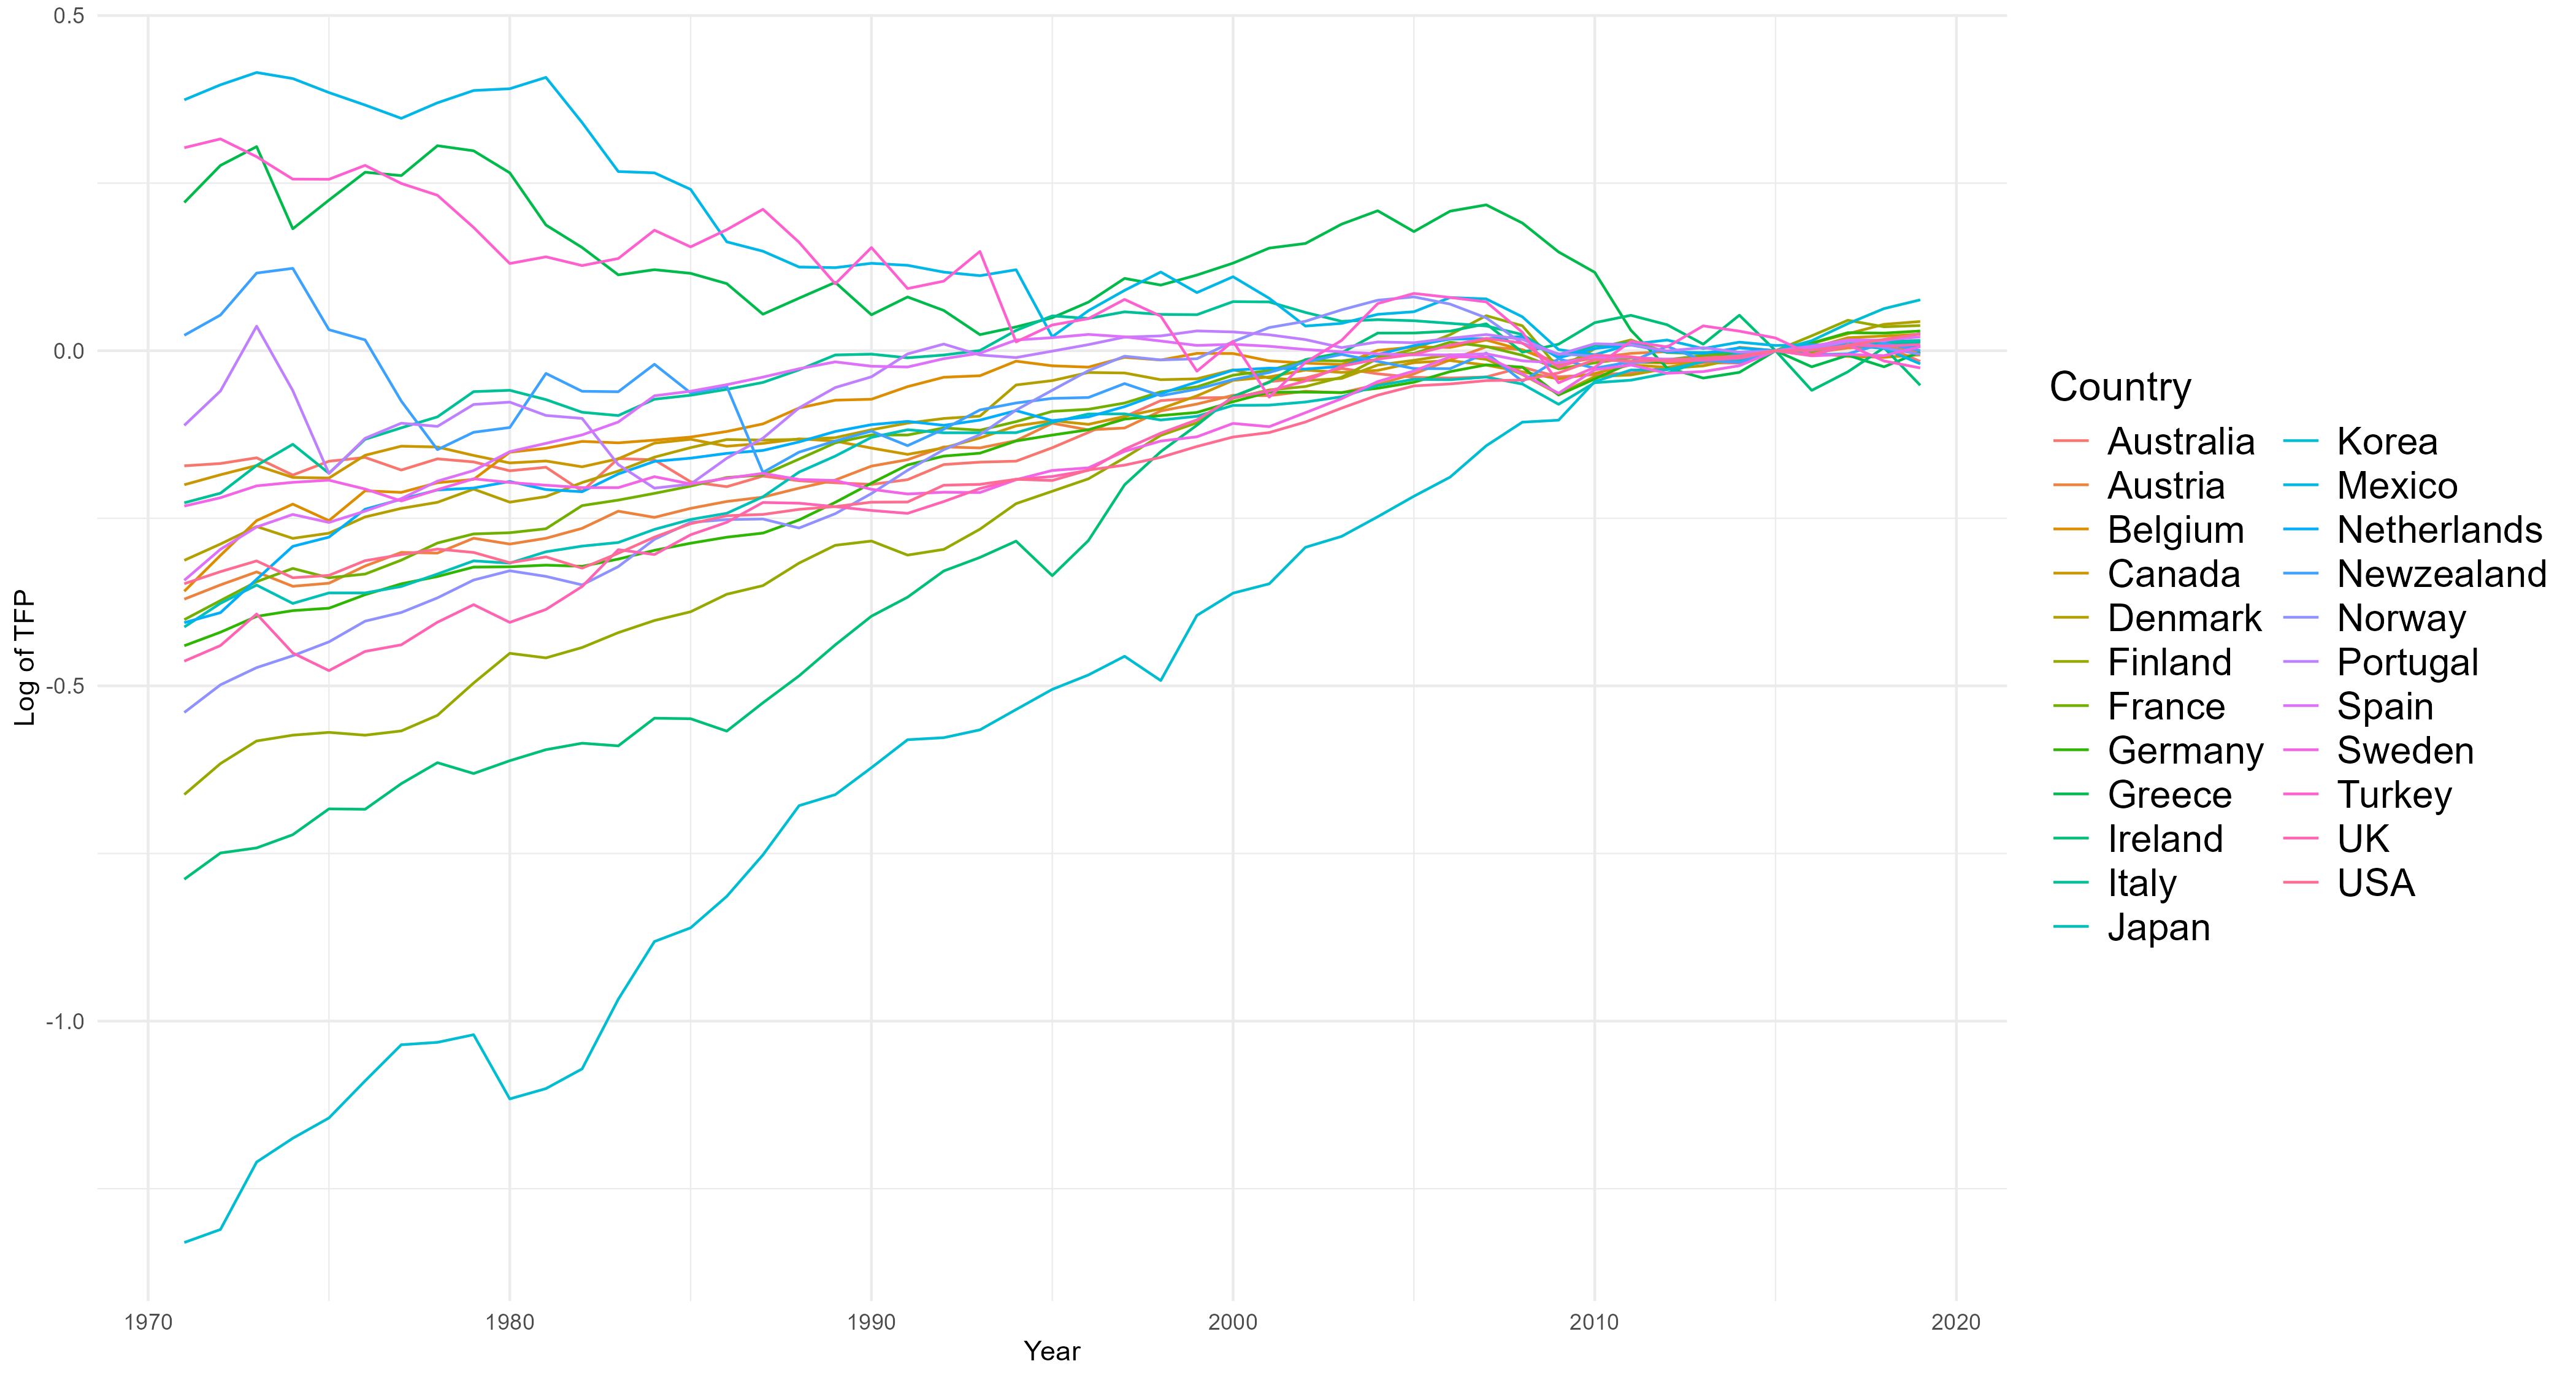
\includegraphics[width=1\linewidth]{TFP.png}
    \label{fig:Trends in Total Factor Productivity}
    \doublespacing
   \justifying{\textit{Figure Notes: TFP for 2015 being indexed to 100. The natural log of the variable is presented in the graph. Source: Author}}
\end{figure}

The summary statistics in Table \ref{table:Summmary statistics} reveal the dynamic evolution of the variables over time. For instance, by 2019, the TFP of Korea, Ireland, and Finland more than doubled compared to their 1971 levels, while TFP declined in Greece, Mexico, New Zealand, and Turkey. This pattern is consistent with the findings of \citet{Coe2009} in their 34-year sample. Such stark contrasts contribute to the cross-country variation in the data. However, Figure \ref{fig:Trends in Total Factor Productivity} shows that most countries in the sample exhibit a positive trend in TFP. Additionally, Table \ref{table:Summmary statistics} highlights that over a longer time period, the variability in countries' import intensities is more pronounced than in the 34-year period analyzed by \citet{Coe2009}. This increased variability allows for a deeper exploration of within-country non-linearities in R\&D spillovers, which will be discussed in subsequent sections. It is important to note that the import intensities reported here account only for imports from the other 22 countries in the sample. By focusing exclusively on intra-sample imports, this study controls for external factors that might otherwise influence the results.

\begin{figure}[h!]
    \centering
    \caption{R\&D Stocks}
     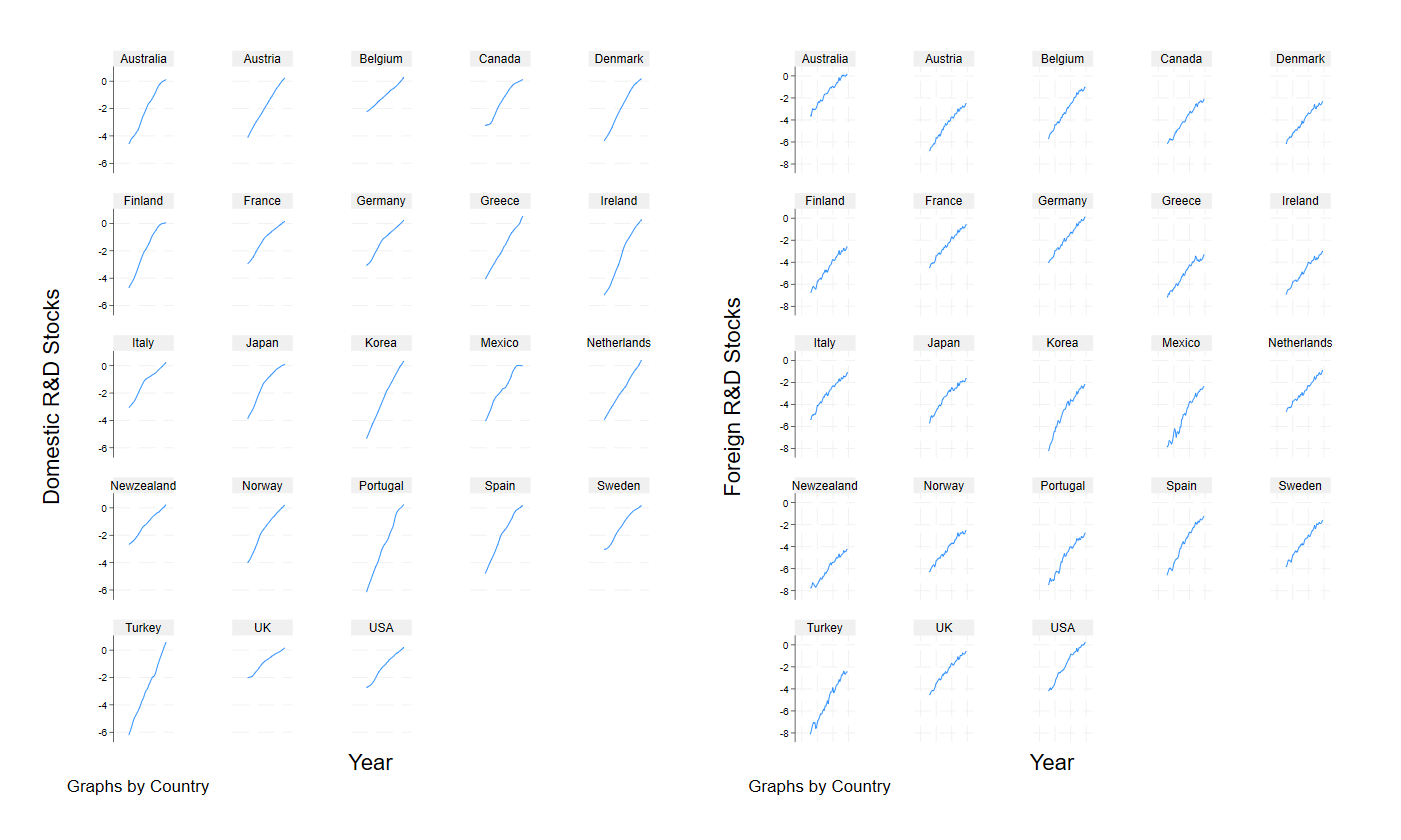
\includegraphics[width=1\linewidth]{R&D Stocks.png}
    \label{fig:KS}
    \textit{Figure Notes: Domestic R\&D stocks $(S^d)$ and Foreign R\&D stocks $S^{f:lp}$ in natural logarithms. Source: Author}
\end{figure}

Compared to TFP, Figure \ref{fig:KS} illustrates that the evolution of both domestic and foreign R\&D stocks exhibits greater variation across countries and over time. There is a marked increase in domestic R\&D stocks in countries such as Australia, Denmark, Finland, Ireland, Korea, the Netherlands, Portugal, Spain, and Turkey. In contrast, domestic R\&D stocks in countries like Belgium, the UK, and the USA start at a high level but show limited growth over the 49-year period.

Foreign R\&D stocks also start at low levels and increase rapidly over time. However, foreign R\&D stocks display greater variation across countries and time compared to domestic R\&D stocks in the selected sample. This observation contrasts with \citet{Coe2009}, who found that their measure of foreign R\&D stocks was more uniform across countries and time. The discrepancy arises because the preferred method of constructing foreign R\&D stocks in this study is the \citet{Lichtenberg1998} method, which uses the GDP of the exporting country in its weighting scheme rather than bilateral import weights. The differences in GDP across countries and over time lead to greater variation in foreign R\&D stocks.

\begin{figure}[h!]
    \centering
    \caption{Heatmap Representing Import Intensities (Total Imports 1971-2019)}
    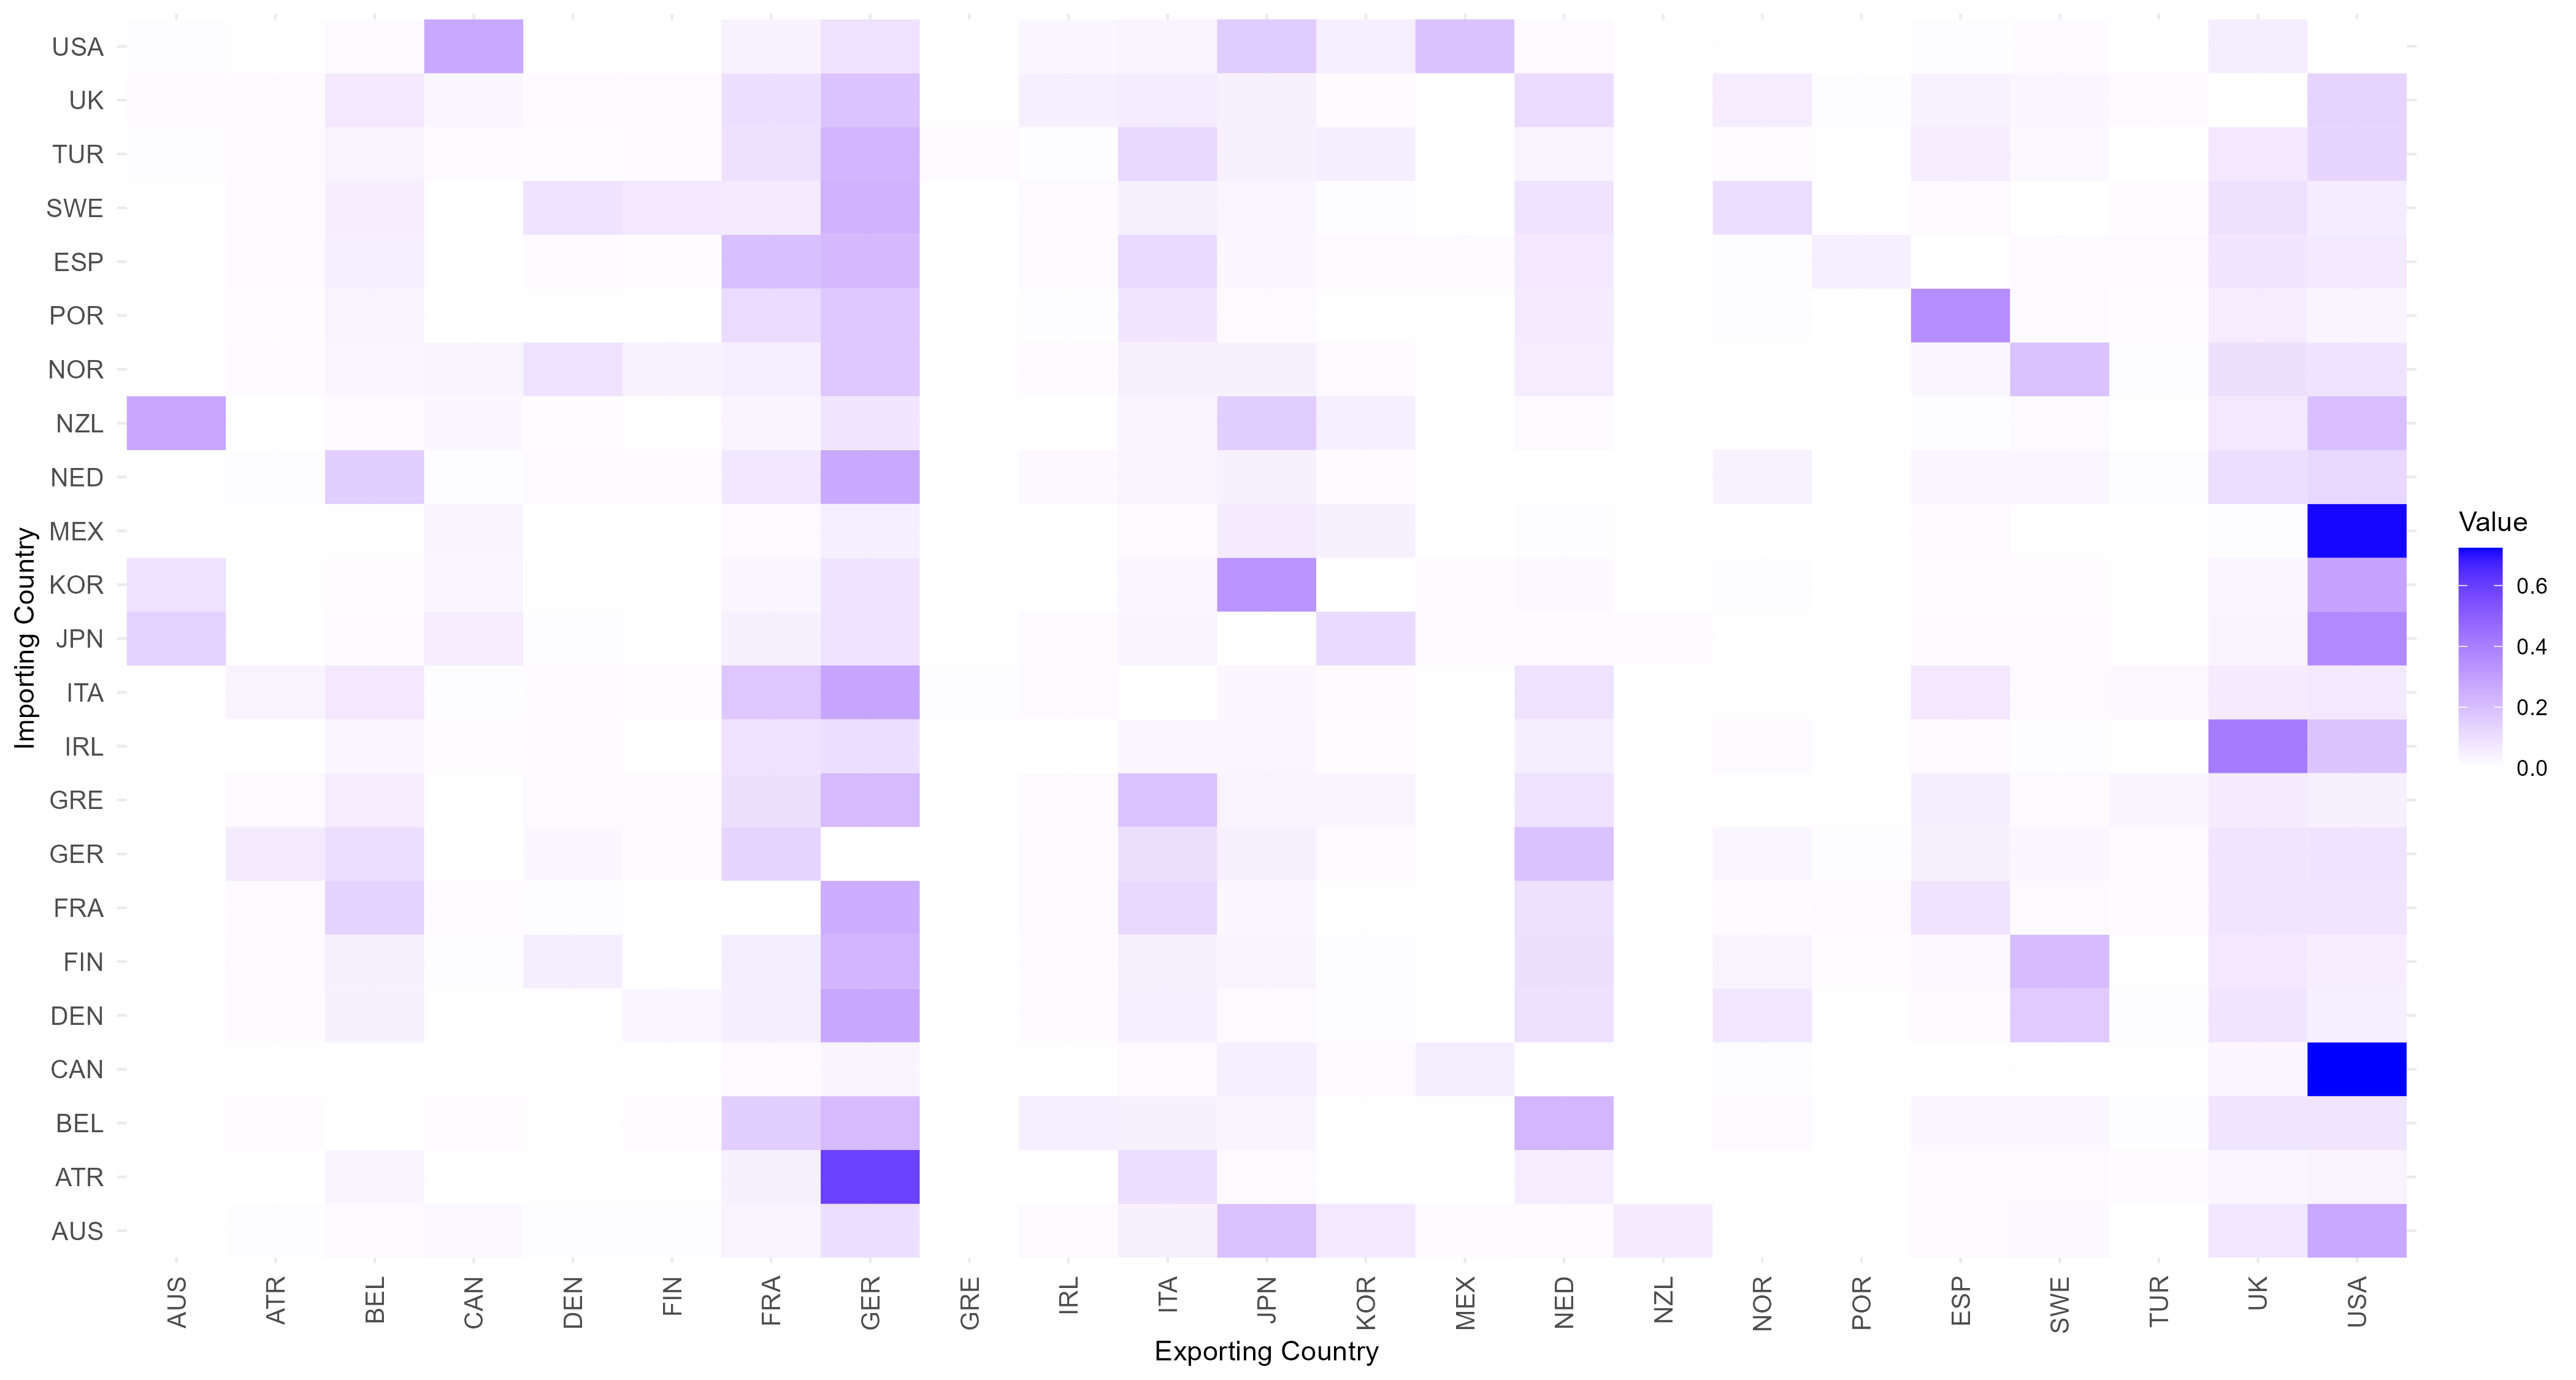
\includegraphics[width=1\linewidth]{heatmap.png}
    \label{fig: heatmap}
    \doublespacing
    \justifying{\textit{Figure Note: Heatmap representing varying intensities of imports from different trade partners.}}
\end{figure}

The impact of trade patterns on R\&D spillovers has been a subject of debate in the literature. \citet{Fracasso2015} show that trade patters have a significant impact through bilateral trade flows. Furthermore, \citet{Acharya2008} demonstrate that although import competition may reduce productivity, high-technology imports from countries closer to the technological frontier can induce higher spillovers, leading to a positive net effect. Figure \ref{fig: heatmap} illustrates that countries import from different partners with varying intensities, which can influence the heterogeneity in R\&D spillovers due to the level of technological advancement in the exporting country.

\section{Empirical Framework}

Existing studies on R\&D spillovers often assume cross-sectional independence of errors, with their econometric models failing to account for contemporaneous correlations arising from common unobserved shocks. \citet{Eberhardt2013} found that neglecting these shocks can lead to biased estimates of R\&D returns, indicating that unobserved shocks and spillovers significantly influence these R\&D coefficients. Therefore, the present study examines the effects of domestic and foreign R\&D stocks on TFP using models that explicitly account for unobserved common shocks and spillovers.

The Common Correlated Effects (CCE) estimator following \citet{Chudik2015} is particularly suited for this analysis, as it is resilient to unit root properties, captures unobserved common effects, handles heterogeneous impacts across units, and supports dynamic modelling. The baseline specification of interest is a growth equation characterised by total factor productivity being a function of domestic and foreign R\&D stocks:
\begin{equation}
TFP_{i,t}=\beta^d_i S_{i,t}^{d} + \beta^f_i S_{i,t}^{f} + u_{i,t}
\label{eq: ccemg}
\end{equation}
\begin{equation}
u_{i,t}=\alpha_i + \lambda_i \textit{\textbf{l}}_t + \epsilon_{i,t}
\label{eq: ucf}
\end{equation}
where $TFP$ is total factor productivity, and $S^d$ and $S^f$ are domestic and foreign R\&D stocks respectively, and all variables are taken in their natural logarithms. The coefficients $\beta^d$ and $\beta^f$ are allowed to differ across countries, which is the salient feature of this empirical strategy. Equation \ref{eq: ucf} shows the multi-factor error structure of $u_{i,t}$, where $\alpha_i$ represents the country-specific fixed effects that capture unobserved time-invariant heterogeneity across countries. The term $\lambda_i \textit{\textbf{l}}_t$ denotes the unobserved common factors, where $\textit{\textbf{l}}_t$ is a vector of common shocks affecting all countries at time $t$, and $\lambda_i$ is a vector of factor loadings that measure the sensitivity of each country to these common shocks. Finally, $\epsilon_{i,t}$ is the idiosyncratic error term that captures the variability that is unexplained by the other components. 

This multi-factor error structure is crucial as it captures unobserved shocks that affect multiple countries simultaneously. By incorporating common factors, the model accounts for common shocks allowing for isolation of the impact of domestic and foreign R\&D stocks from these overarching influences. The factor loadings $\lambda_i$ enable the model to account for the varying impact of common shocks across countries, recognising that different countries may respond differently to the same global event. This approach improves estimation accuracy by addressing cross-sectional dependence, leading to more accurate and consistent estimates of the coefficients $\beta^d$ and $\beta^f$.

To ensure robustness and comparability, the study begins by applying the \citet{Pedroni2004} DOLS model. This is done for two reasons: first, to determine if the extended panel of 49 years yields results consistent with prior research, notably \citet{Coe2009}; and second, to facilitate a comparison of models assuming cross-sectional independence with those accounting for cross-sectional dependence. The DOLS results serve as a benchmark before proceeding to more sophisticated models. 

\subsection{Dynamic Linear Specifications}

Due to the importance of using a dynamic analysis when dealing with panels with a large time-dimension, this study uses an error correction representation of the baseline specification. \citet{Eberhardt2015} point towards three reasons why an error correction specification is superior to static or restricted dynamic models: (a) they distinguish between short-run and long-run relationships; (b) they allow inferences of the speed of adjustment of the model in response to an exogenous shock in the previous period; (c) in the case of mixed order of variables, the statistical significance of the error correction term is evidence of an equilibrium long-run relationship between the selected variables. The error correction representation of the specified model is as follows:
\begin{align}
    \Delta TFP_{i,t} &= \alpha_i + \upsilon_i(TFP_{i,t-1} - \beta_i^d S_{t-1}^d - \beta_i^f S_{t-1}^f - \lambda_i \textit{\textbf{l}}_{t-1}) \notag \\
    &\quad + \gamma_i^d \Delta S_t^d + \gamma_i^f \Delta S_t^f + \gamma_i^l \Delta \textit{\textbf{l}}_t + \epsilon_{i,t} \label{eq: LR}
\end{align} 
$\beta_i^d$ and $\beta_i^f$ in Equation (\ref{eq: LR}) represent the long run relationship between TFP and stocks of domestic and foreign R\&D respectively, and $\gamma_i^d$ and $\gamma_i^f$ represent the short run relationships. $\upsilon_i$ signifies the speed of adjustment of the model to its long run equilibrium. Equation (\ref{eq: ECM}) is a reparameterisation of Equation (\ref{eq: LR}).
\begin{align}
    \Delta TFP_{i,t} &= \pi_{0i} + \pi_i^{EC} TFP_{i,t-1} + \pi_i^d S_{t-1}^d + \pi_i^f S_{t-1}^f + \pi_i^l \textit{\textbf{l}}_{t-1} \notag \\
    &\quad + \mu_i^d \Delta S_t^d + \mu_i^f \Delta S_t^f + \mu_i^l \Delta \textit{\textbf{l}}_t + \epsilon_{i,t} \label{eq: ECM}
\end{align}
In Equation (\ref{eq: ECM}), $\pi_i^{EC}$ shows the speed at which the economy converges to its long-run equilibrium. The long run coefficients can be calculated as $\beta_i^d=-\pi_i^d/\pi_i^{EC}$ and $\beta_i^f=-\pi_i^f/\pi_i^{EC}$.
 
According to \citet{Pesaran2006}, the CCE model entails taking cross-sectional averages of all variables included in the model. However, \citet{Chudik2015} have highlighted the vulnerability of this approach to small sample bias, which is especially obvious in dynamic panels with modest time series dimensions. This calls into question the consistency of the original \citet{Pesaran2006} paradigm. To overcome these concerns, it is advised that additional lags be added to the cross-section averages of all model variables. 
\begin{align}
    \Delta TFP_{i,t} &= \pi_{0i} + \pi_i^{ECT} TFP_{i,t-1} + \pi_i^d S_{i, t-1}^d + \pi_i^f S_{i, t-1}^f + \mu_i^d \Delta S_{i,t}^d  + \mu_i^f \Delta S_{i,t}^f \notag \\
    &\quad + \tau_i^{\Delta TFP} \overline{\Delta TFP}_{t} + \tau_i^{TFP} \overline{TFP}_{t-1} + \tau_i^d \overline{S^d}_{t-1} + \tau_i^f \overline{S^f}_{t-1}+ \rho_i^d \overline{\Delta S^d_t}  \notag \\
    &\quad + \rho_i^f \overline{\Delta S^f_t} + \sum_{p=0}^P \varphi_i^{\Delta TFP} \overline{\Delta TFP}_{t-p} + \sum_{p=1}^P \varphi_i^d \overline{\Delta S^d}_{t-p} + \sum_{p=1}^P \varphi_i^f \overline{\Delta S^f}_{t-p} \notag \\
    &\quad  + \varepsilon_{i,t} \label{eq:tfp}
\end{align}
Equation (\ref{eq:tfp}) is the complete specification of the error correction model given by \citet{Chudik2015}, who demonstrate that when augmented with an adequate number of lagged cross-section averages ($P=int(\sqrt[3]{T})$ lags is proposed as a rule of thumb \citep{Eberhardt2015}), the CCEMG estimator exhibits strong performance even within a dynamic model featuring weakly exogenous regressors. Hence, the number of lagged cross-sectional averages is set to $P=int(\sqrt[3]{49})=int(3.659)=3$.

To analyze parameter heterogeneity, country-specific coefficients are plotted against economic size using G7 categorisation as a proxy, following \citet{Coe1995}. It is expected that G7 countries will exhibit higher coefficients for domestic R\&D, while non-G7 countries will show higher coefficients for foreign R\&D. Additionally, heterogeneity based on human capital is examined following \citet{Coe2009}, and on the basis of imports, in line with \citet{Lichtenberg1998}. This analysis aims to identify the differential impacts of domestic and foreign R\&D across countries with varying levels of development, human capital, and trade openness. 

\subsection{Non-Linear Static Model}

This study hypothesises an inverted U-shaped relationship between R\&D stocks and productivity, justified using the escape-competition and Schumpeterian effects characterised by \citet{Aghion2005}. It is expected that both domestic and foreign stocks of R\&D will have a diminishing effect on productivity as imports increase. To test this hypothesis, this study uses an interaction of R\&D stocks and import share of GDP to assess non-linearities based on import intensity.
\begin{equation}
TFP_{i,t}=\beta^d S_{i,t}^{d} + \beta^f S_{i,t}^{f} + \beta^{md} m_{i,t} S_{i,t}^{d} +  \beta^{mf} m_{i,t} S_{i,t}^{f} + \lambda_i \textit{\textbf{l}}_t + u_{i,t}
\label{eq: nl}
\end{equation}

Based on the Equation (\ref{eq: nl}), this study makes statistical inferences about the presence on non-linearities using the static CCE model rather than a dynamic one, because the inclusion of cross-sectional dependence and parameter heterogeneity in an error correction specification would introduce a level of complexity that extends beyond the scope of this analysis. A threshold of 15\% is used to disaggregate the panel\footnote{15\% is the average of the country-wise mean import intensity, excluding outliers.} into a low import regime and a high import regime. It is, however, challenging to tie spillover effects to specific import thresholds, just as it would be unreasonable to assert that economic growth will be steady at 14\% imports-to-GDP ratio but significantly worse at 16\% (adapted from \citet{Eberhardt2015}). The connection between R\&D stocks and economic growth is intricate, and identifying a precise threshold that leads to a growth deceleration requires considering various country-specific factors. Therefore, this study also examines the heterogeneity in non-linearity thresholds across the sample of countries.


\section{Results and Discussion}

This study carries out the cross sectionally augmented Im-Pesaran-Shin \citep{Pesaran2007} test for testing panel unit-roots and the \citet{Pesaran2004} test to detect cross-sectional dependency in the variables (see Appendix \ref{ap: A}). The results suggest mixed order of integration and considerable cross-sectional dependence among the variables. Furthermore, results of the \citet{Westerlund2007} cointegration tests reveal evidence of a long-run equilibrium relationship between the variables (see Appendix \ref{ap: A}). To demonstrate the replicability of the results with respect to previous studies, and to show the superiority of models that account for unobserved common shocks, this study first presents the results of DOLS model.

\subsection{Dynamic OLS}

\begin{table}[h!]
    \caption{Panel Dynamic OLS} 
    \centering
    \doublespacing
    \setlength{\tabcolsep}{0.7pt}
    \begin{tabular*}{\linewidth}{@{\extracolsep{\fill}} l c c c c}
        \hline
        Variables & (1) & (2) & (3) & (4) \\
        \hline
        $S^d$ & 0.052*** & 0.041*** & 0.024*** & 0.063 \\
          & (8.092) & (3.782) & (-4.073) & (0.996) \\
        $S^{f}$ & 0.054*** &  &  0.141***  &  \\
         & (-4.087) &  & (13.00) & \\
        $m*S^{f}$ &  & 0.040*** &  & -0.197***  \\
         &  &  (9.557) &  &  (-13.130)  \\
        $H$ & &  &  0.285*** & 0.273**\\
         &  &  &  (-7.125) & (3.710)  \\
        \hline
    \end{tabular*}
    \justifying{\textit{Table Notes: DOLS results based on a sample of N=23 countries. t-statistics reported in parentheses. $TFP$, $S^{d}$, and $S^{f}$ are taken in natural logarithms, and $m=Imports_{it}/GDP_{it}$. *, **, and *** represent statistical significance at the 10\%, 5\%, and 1\% level respectively.}}
    \label{table: DOLS}
\end{table}

For the baseline model, this study begins by attempting to replicate the results of the baseline specification given by \citet{Coe2009} using the dynamic OLS (DOLS) method. In doing so, this study attempts to understand whether extending the time frame from the 34 years taken by \citet{Coe2009} to 49 years significantly changes the magnitude of coefficients obtained for domestic and foreign R\&D stocks.

In Table \ref{table: DOLS}, columns (1) to (4) replicate the baseline specification as in \citet{Coe1995}, where specifications (3) and (4) use the human capital as a control variable. The statistically significant positive coefficients for $S^{f}$ and $mS^{f}$ in specification (2) shows that R\&D spillovers are stronger as import share of GDP increases, following the results of \citet{Lichtenberg1998}. Furthermore, the regression results in column (1) and (3) yields a higher coefficient for foreign R\&D stocks than \citet{Coe2009}. However, when the interaction terms are used controlling for human capital (specification (4)), foreign R\&D stocks have a negative and significant coefficient, which is completely contrary to the findings of \citet{Coe2009}. It shows that as import intensity increases, R\&D spillovers decline. This is the first sign of evidence in favour of the argument that when a longer time frame is used, increasing imports intensity may cause spillovers to decline. The positive coefficients in three out of four specifications demonstrates that when the panel used by \citet{Coe2009} is extended to 49 years, the results are still in line with empirical literature.

\subsection{Error Correction Models}
The results of the DOLS model in the previous subsection is, for the most part, in line with the existing literature on the subject. However, due to mixed order of integration among the variables, it is best to use error correction models, which are resilient to unit-root properties of the variables \citep{Engle1987}. Auxiliary error-correction models presented in Appendix \ref{ap: C} show that models with heterogeneous coefficients that use a multi-factor error structure are the most successful in minimising residual cross-sectional dependence.

\begin{table}[htbp!]
    \centering
    \doublespacing
      \setlength{\tabcolsep}{0.75pt} 
        \caption{Linear Dynamic ECM (2 Lags)}
            \fontsize{11}{12}\selectfont
  \begin{tabular*}{\textwidth}{@{\extracolsep{\fill}}l*{6}{c}}
    \hline
    Variables & \multicolumn{2}{c}{Full Sample} & \multicolumn{2}{c}{G7} & \multicolumn{2}{c}{Non-G7} \\
    \cmidrule(lr){2-7}
        & (1)  & (2) & (3) & (4) & (5) & (6)  \\
         \hline
        Domestic R\&D  \\
       \textit{LRA} & 0.061** & 0.046  & 0.117***  & 0.193** & 0.034 & -0.029 \\
         & (0.030)  & (0.056) &  (0.036) & (0.087) & (0.036) & (0.055) \\
         \textit{ALR} & 0.233 & 0.005  & 0.094** & 0.058 & 0.294 & -0.017  \\
         & (0.231)  & (0.075) & (0.048)  & (0.201) & (0.334) & (0.068) \\
        Foreign R\&D  \\
        \textit{LRA} & 0.035 & 0.008 & 0.030 & 0.032**  & 0.038 & -0.004 \\
         & (0.026) & (0.007) & (0.029) & (0.013) & (0.037) & (0.049) \\
        \textit{ALR} & -0.370 & 0.014 & -0.001 & 0.044 &  -0.531 & 0.001\\
         & (0.420) & (0.007) & (0.050) & (0.032) &  (0.606) & (0.058) \\
         Human Capital\\
         \textit{LRA} &  & 1.015 &  & 0.205 &  & 1.429 \\
         &  & (1.255) &  & (2.404) &  & (1.487) \\
        \textit{ALR} &  & -0.183 &  & -1.615 & & 0.443 \\
         & & (0.007) &  & (2.655)  & & (1.255) \\
        $ECT_{t-1}$ & -0.457*** & -0.684*** & -0.499*** & -0.759***  & -0.439*** & -0.650***\\
         $t$-statistic & -7.95 & -8.71 & -3.38 & -3.33 & -7.91 & -10.76 \\
         $\overline{t}$-statistic & -3.17 & -3.65 & -3.49 & -3.94 & 3.037 & -3.521 \\
         \hline
         Observations& 1058 &  1058 & 322 & 322 & 736 & 736 \\
         $CD$& -2.34 & 1.48 & -0.37 & -0.25 & -2.26 & -1.66 \\
         $RMSE$& 0.011 & 0.009 & 0.006 & 0.004 & 0.013 & 0.011 \\
         \hline
    \end{tabular*}
     \fontsize{11.5}{12}\selectfont
        \justifying{\textit{Table Notes: The initial set of t-statistics for the ECT are calculated from the coefficients specific to each country, following \citet{Pesaran1995}. The second set reflects the mean of the t-statistics obtained across different countries. The significance of the Error Correction Term (ECT) is assessed according to the method described by \citet{Gengenbach2016}. RMSE is the root mean squared error; CD test reports the \citet{Pesaran2004} test. *, **, and *** represent statistical significance at the 10\%, 5\%, and 1\% respectively.}}
    \label{tab: CCEBase}
\end{table}

The specifications presented in Table \ref{tab: CCEBase} use three lagged cross-sectional averages is used to ensure correct specification of the error structure. Each model emphasises the error correction term coefficient and the long-run estimates to examine cointegration and identify evidence of a long-run relationship. This approach (i) initially calculates the long-run coefficient for each country, which is subsequently averaged (ALR)\footnote{Note that the average long-run coefficient is very sensitive to positive outliers in the group-specific EC-coefficients.}, and (ii) first averages the ECT coefficients and then determine the long-run average (LRA). This empirical strategy is inspired by \citet{Eberhardt2015}. 

In the CCEMG models presented in Table \ref{tab: CCEBase}, the error correction terms are statistically significant, which is evidence of an equilibrium long-run relationship between the variables. Furthermore, with the exception of specifications (1) and (5), the CD statistic of the residual term shows cross sectional independence, which proves that the error process is correctly specified; common shocks like war \citep{Moretti2023} and indirect spillovers elaborated by \citet{Keller2010} and \citet{lumenga2005} have been sufficiently captured. 

The findings of the CCEMG model for the full sample reveals a positive and statistically significant long-run average coefficient for domestic R\&D stocks, which turns insignificant when human capital is used as a control. The long run average coefficients are statistically significant in both specifications for the sub-sample of G7 countries\footnote{The specifications for subsamples utilize the cross-sectional averages of all countries in the full sample, ensuring that the results are comparable across different group subsets.}, with a coefficient higher than the coefficients reported in the DOLS model in Table \ref{table: DOLS} and the results of \citet{Coe2009}. However, the coefficient for the long-run average effect for non-G7 countries are statistically insignificant; in fact, for the model controlling for human capital, the coefficient is negative. An explanation for these findings is that large countries engage in a variety of R\&D activities, allowing them to more effectively leverage available complementarities \citep{Coe1995}. On the other hand, smaller countries invest more in adoption of foreign technology, rather than innovating their own \citep{Santacreu2015}; hence, one may expect non G7-countries to have a larger coefficient for foreign R\&D stocks. However, the results of the models find no such evidence; the coefficients for foreign R\&D stocks yield statistically insignificant coefficients. Here, insignificant coefficients do not indicate that significant effects are absent; instead, it emphasises the heterogeneity among countries, with varying dynamics, that tend to cancel each other out on average. Such heterogeneity arises because the ability to harness tacit knowledge and a country's rate of innovation and growth depend on its prior research experience and successes \citep{Mancusi2008}, domestic institutions \citep{Coe2009}, and human capital \citep{Kneller2006}.

This study explores heterogeneity in country-level coefficients that stems from three sources. First, \citet{Coe1995} found that in smaller countries, foreign R\&D capital stock might be as crucial as domestic R\&D capital stock, whereas in G7 countries, domestic R\&D capital stock may hold greater significance. Second, \citet{Nelson1966} suggests that human capital affects the level and intensity of technology diffusion by influencing a country's capacity to absorb foreign knowledge. In this regard, \citet{Coe2009} find that countries with higher tertiary education levels have significantly larger coefficients for foreign R\&D stocks. Finally, import intensity may influence heterogeneity and potential non-linearities in country coefficients. \citet{Lichtenberg1998} argue that foreign R\&D capital stocks have stronger effects on due to higher import intensity, a result corroborated by various other studies (see for e.g. \citet{Coe2009} and \citet{Madsen2007}).

\begin{figure}[h!]
    \centering
    \doublespacing
        \caption{Heterogeneity Based on Economic Size and Human Capital}
    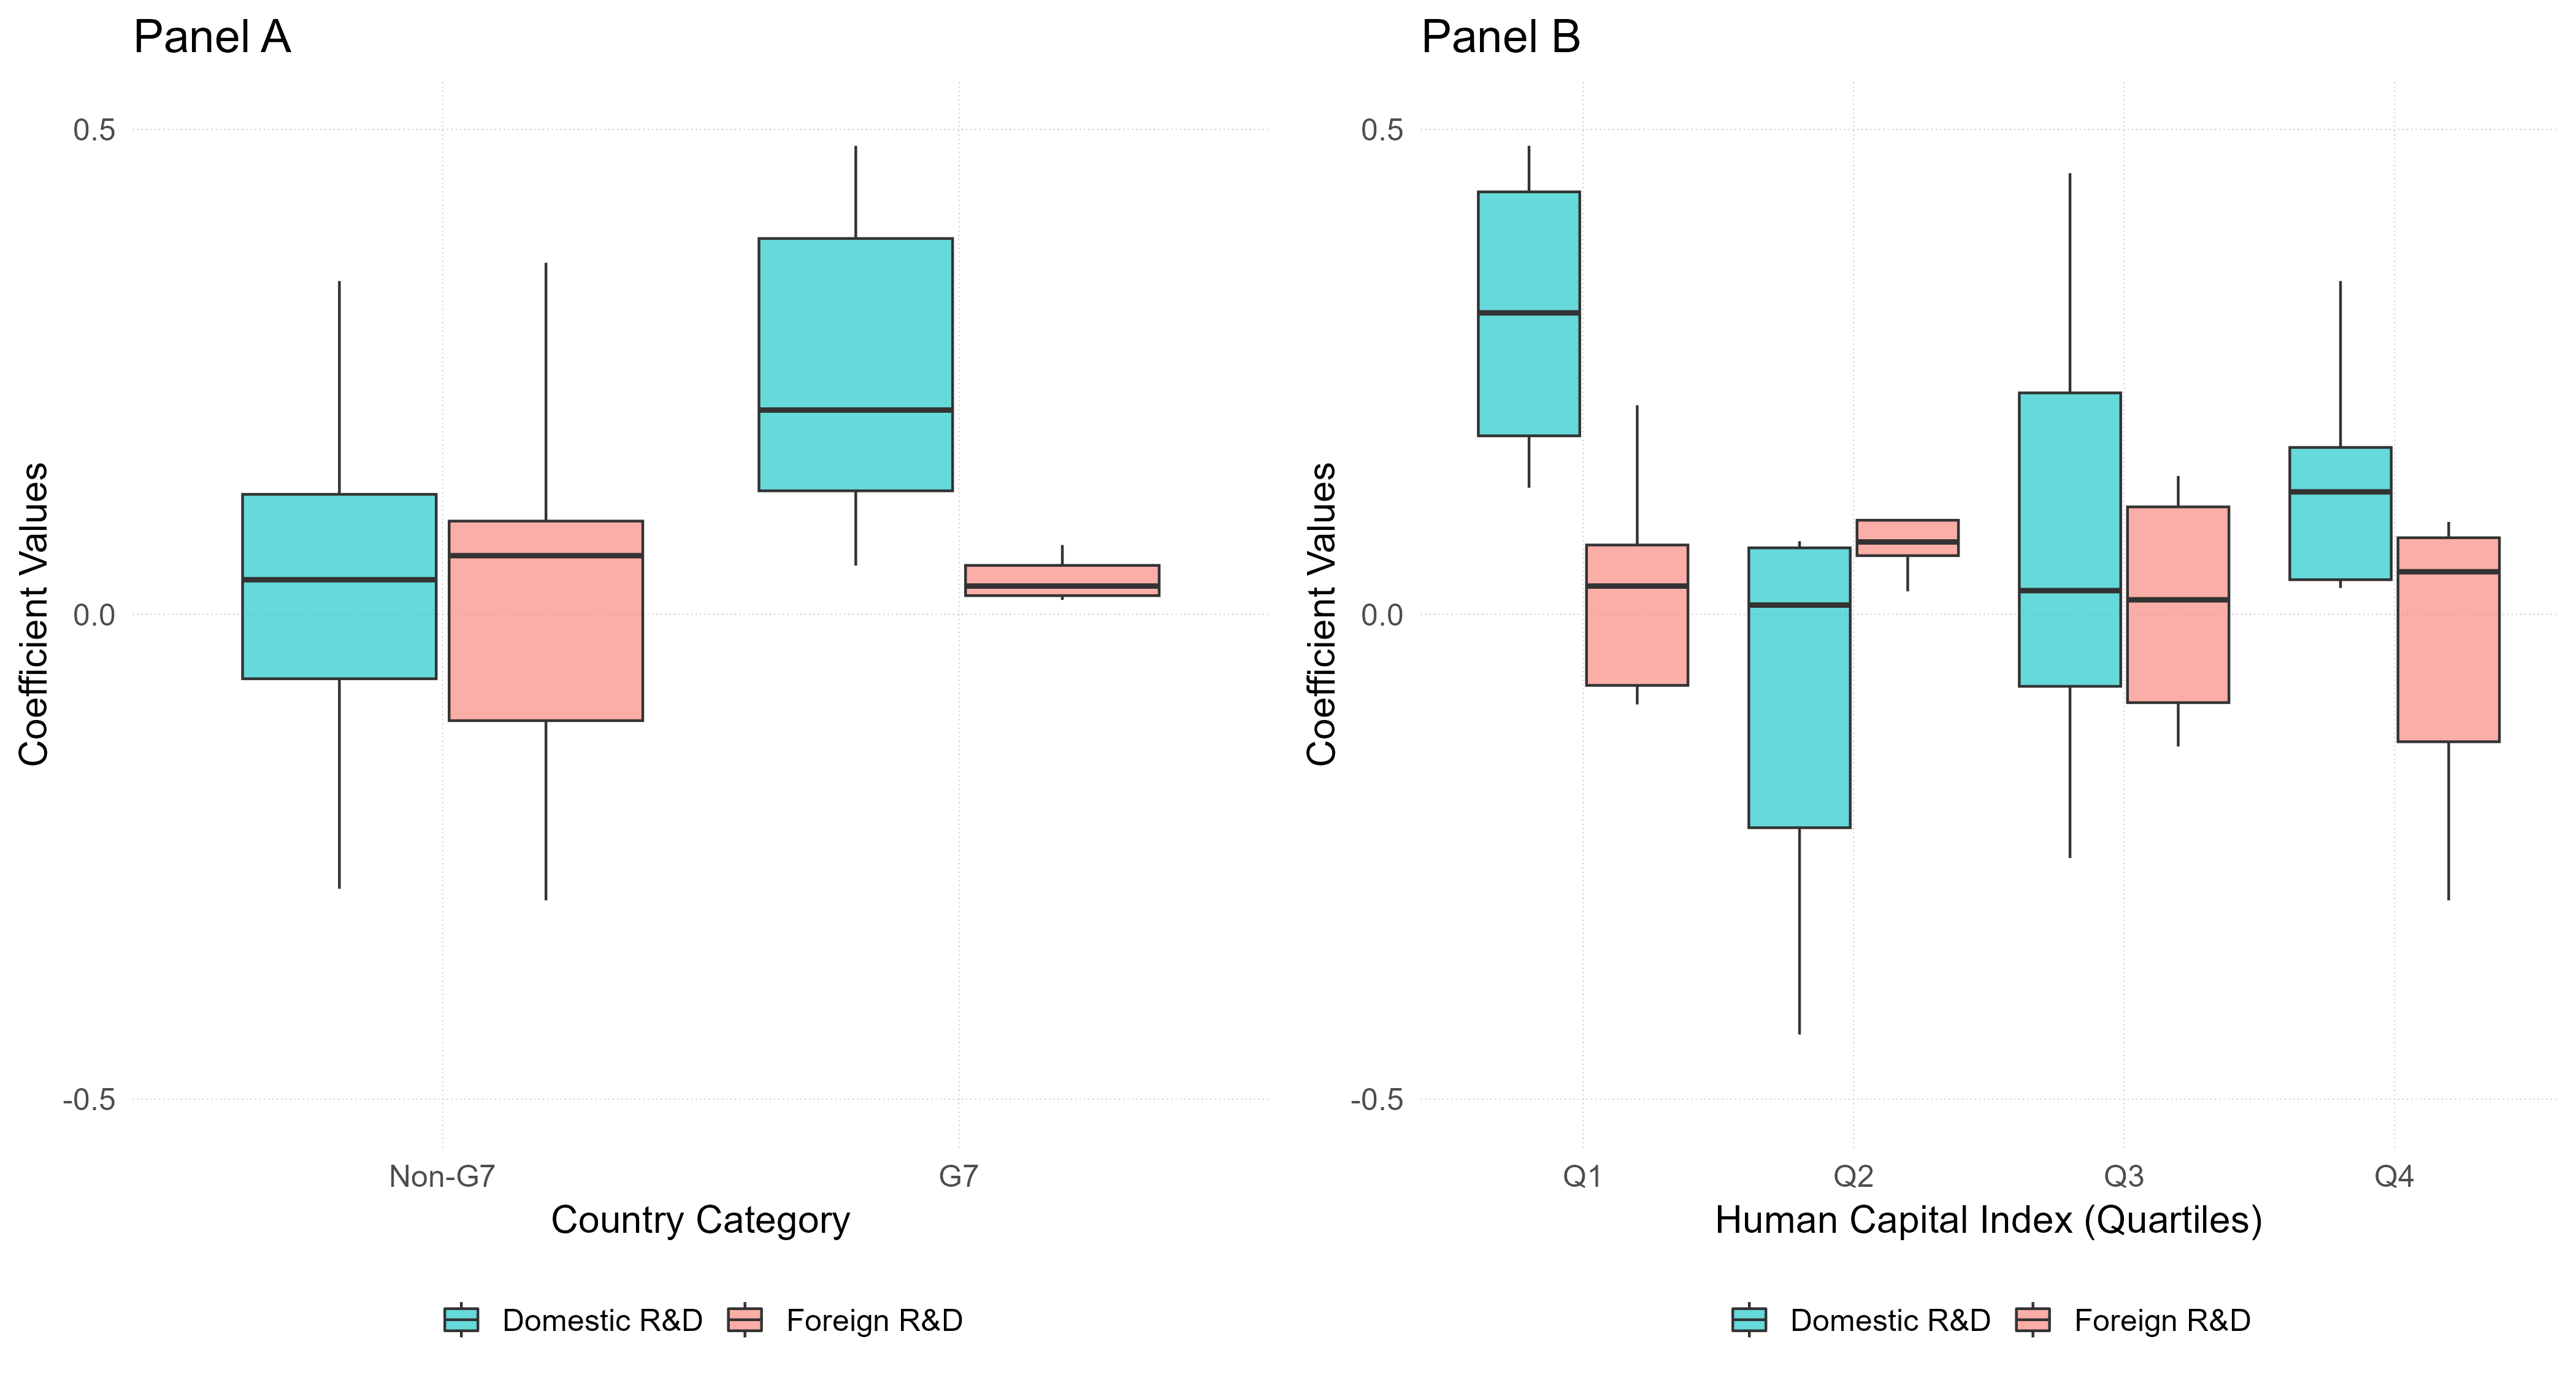
\includegraphics[width=1\linewidth]{boxplots.png}
    \label{fig: boxplots}
    \justifying{\textit{Figure Notes: The boxplot uses country specific coefficients of specification (2) of the CCEMG model in Table \ref{tab: CCEBase}. Panel A classifies the countries into G7 and non-G7 countries. Panel B classifies countries based on their human capital index into quartiles: Q1 being countries with the highest human capital and Q4 being the lowest}}
\end{figure}

Panel A of Figure \ref{fig: boxplots} reveals that when the sample classified into G7 and non-G7 countries, domestic R\&D stocks appear to have a higher coefficient, on average, for countries in the G7. Furthermore, Panel A of Figure \ref{fig: boxplots} also reveals that in non-G7 countries, domestic R\&D is just as important as foreign R\&D in determining productivity, whereas in G7 countries, domestic R\&D stocks are more important. This is in line with the results of \citet{Coe1995} and \citet{Engelbrecht1997}, who find similar evidence, but in contrast with the results found by \citet{Coe2009}, who report that countries in the G7 have a lower coefficient for domestic R\&D stocks.

Panel B of Figure \ref{fig: boxplots} shows a higher coefficient for domestic R\&D stocks for countries in the top quartile of human capital, but no visible differences in the coefficients of domestic and foreign R\&D stocks for countries in the three other quartiles. The higher coefficients for domestic R\&D capital in countries with the largest index of human capital reflects higher skill levels and technical ability of workers in these countries. However, in contrast to the theoretical predictions of \citet{Benhabib1994} and the empirical evidence of \citet{Coe2009}, differences in human capital is not a major source of heterogeneity in R\&D spillovers. The justification for failure to observe heterogeneity is that using particular technology builds technology-specific expertise, and diminishes the motivation to adopt new technologies, as switching would mean forfeiting the benefits derived from this accumulated knowledge \citep{Jovanovic1996}. As a result, both workers and firms tend to stick with older technologies, even when potentially superior alternatives are available \citet{Comin2004}. In OECD countries, which are already near the cutting-edge of technological advancement, the focus is on developing and refining domestic technologies, as they experience lower international knowledge spillovers and gain higher significant returns from domestic R\&D efforts.

\begin{figure}[ht!]
    \centering
    \doublespacing
    \caption{Heterogeneity Based on Import Intensity}
    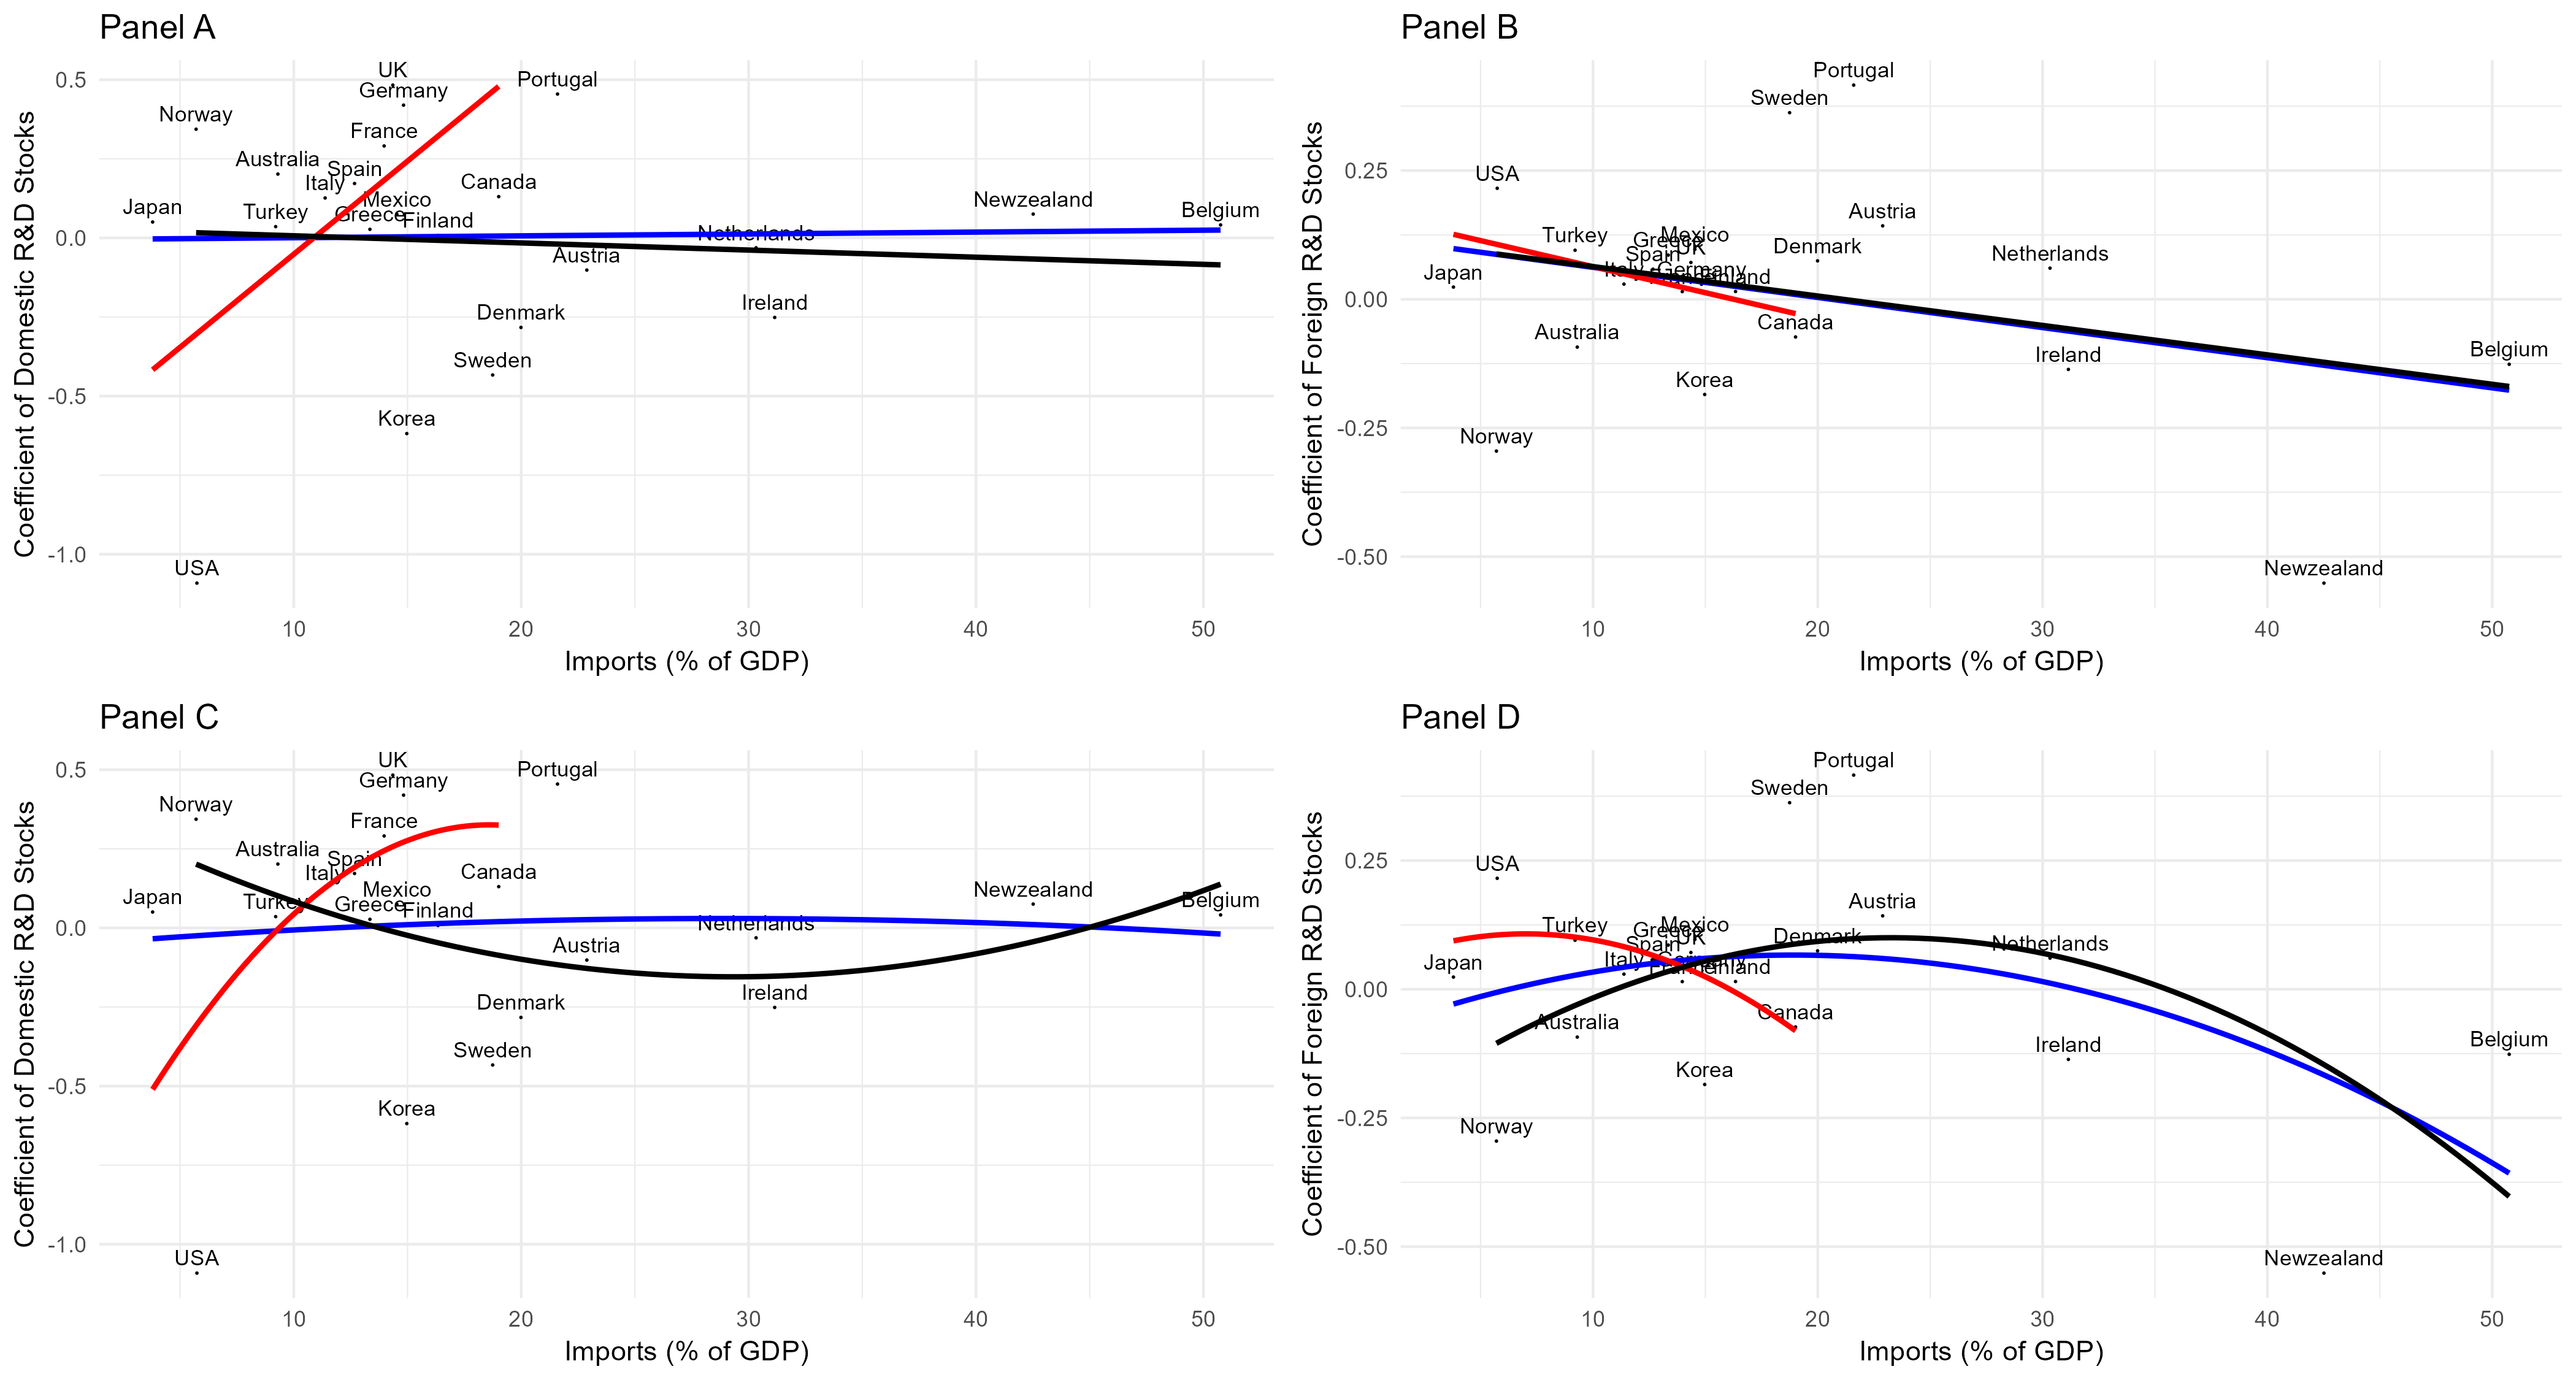
\includegraphics[width=1\linewidth]{HC_IMP.png}
    \label{fig: imp}
    \justifying{\textit{Figure Notes: Panels A and B show the linear plot of country specific coefficients of domestic and foreign R\&D stocks respectively, whereas Panels C and D show the polynomial plot. The blue line represents the full sample, the red line represents G7 countries and the black line represents non-G7 countries.}}
\end{figure}

Figure \ref{fig: imp} plots the country specific coefficients against average import intensity. Panels A and C of Figure \ref{fig: imp} show that there is very little heterogeneity in coefficients of domestic R\&D stocks with respect to imports when the entire sample is considered. However, G7 countries appear to experience greater returns to domestic R\&D capital as imports rise. This is because advanced economies are immune to the detrimental impact of higher imports and the consequent domestic competition effects \citep{Aghion2005}. 

Panel B reveals that as average import intensity increases, the coefficient of foreign R\&D stock decreases. This is in contrast with the findings of \citet{Lichtenberg1998} and \citet{Coe2009}, who find that higher import intensity results in higher R\&D spillovers. The effect of import intensity on the coefficient of foreign R\&D stocks is similar for the sub-samples of G7 and non-G7 countries. Panel D of Figure \ref{fig: imp} presents the non-linear plots for country specific coefficients against import intensity. The coefficients for foreign R\&D stocks reveal a clear inverted U-shaped relationship, that is consistent for all sub-samples, in line with the expectations of the earlier established theory through the escaping-competition and Schumpeterian effects given by \citet{Aghion2005}. 

The analysis conducted so far explores whether there is a non-linear relationship between TFP and R\&D stocks mediated by import intensity. Moving forward, the focus will be on empirical models that accommodate both varying long-run relationships across countries and potential threshold effects within individual countries.

\subsection{Non-Linear Static Model}

The hypothesis tested in this section is that the coefficient of R\&D stocks initially rises as domestic firms learn to adapt in response to increased imports (escaping-competition effect), and eventually peaks and falls as firms no longer find it profitable to innovate (Schumpeterian effect). The results in table \ref{tab: nl} use specifications for three sub-samples: the full sample of 23 countries, the sub-sample of countries with an import intensity of less than 15\% (13 countries), and the sub sample of countries with import intensity of greater than 15\% (10 countries).

\begin{table}[h!]
    \centering
     \doublespacing
        \caption{Non-Linear Model}
        \setlength{\tabcolsep}{0.8pt} 
  \begin{tabular*}{\textwidth}{@{\extracolsep{\fill}}l*{6}{c}}
  \hline
    Variables & \multicolumn{2}{c}{Full Sample} & \multicolumn{2}{c}{$m<15\%$} & \multicolumn{2}{c}{$m>15\%$} \\
    \cmidrule(lr){2-7}
        & (1)  & (2) & (3) & (4) & (5) & (6)  \\
        \hline
        $S^d$ & -0.001 & 0.018 & 0.061 &0.082* & -0.094  & -0.110 \\
         & (0.041) &(0.047)  & (0.048) &(0.044) &(0.080)  & (0.063)\\
        $S^f$ & 0.075*** & 0.075*** & 0.061*** & 0.061** & 0.066 & 0.082* \\
         & (0.020) & (0.022) & (0.021) & (0.024) & (0.051) &(0.046) \\
        $m*S^d$ & 0.017 & 0.070  &0.449  &0.336  &0.072  &0.026 \\
         & (0.193) &(0.149)  &(0.292)  &(0.221)  &(0.095)  &(0.115) \\
        $m*S^f$ & -0.050 & -0.055 & -0.388* &-0.286**  &-0.008  &0.029 \\
         & (0.120) & (0.077) & (0.206) & (0.127) & (0.046) & (0.047) \\
         $H$&  &-0.805  &  & -0.246 &  &-0.824 \\
         & & (0.779) & & (0.965) & & (0.681) \\
         \hline
        N & 1127 & 1127 & 637 & 637 & 490 & 490 \\
        CD & -2.51 & -2.81 & -3.88 & -2.90 & -2.39 & -3.28\\
        RMSE & 0.020 & 0.018 & 0.020 & 0.016 & 0.019 &0.016 \\
        \hline
    \end{tabular*}
    \label{tab: nl}
    \justifying{\textit{Table Notes: Standard errors reported in parentheses following \citet{Pesaran1995}. *, **, and *** represent statistical significance at the 10\%, 5\%, and 1\% respectively.}}
\end{table}

In Table \ref{tab: nl}, the coefficient for foreign R\&D ($S^f$) is positive and statistically significant in the full sample and the countries in the low import regime. However, in the high import regime, the coefficient for $S^f$ becomes statistically insignificant. This suggests that while foreign R\&D initially boosts productivity in countries with moderate import levels, its impact diminishes as imports increase. The results also indicate the presence of non-linearities in the low import regime, as demonstrated by the statistical significance of the $m*S^f$ term. This implies that as imports rise, the initial benefits from foreign R\&D may intensify, but at a diminishing rate. Once a country transitions into a high import regime, these non-linearities disappear, likely because the economy has already absorbed much of the available foreign technology, reducing the marginal productivity gains from further imports. At this stage, the returns from foreign R\&D do not diminish further, but the potential for additional knowledge acquisition through imports is also exhausted. These findings suggest evidence of both escaping competition and Schumpeterian effects in countries with low import levels. However, there is no evidence of such non-linearities in domestic R\&D stocks across all sub-samples, or in foreign R\&D stocks within the full sample and the high import regime sub-sample.

The non-linear coefficients of the full-sample mean group model can be used to identify turning points or country specific import thresholds, beyond which the direction of R\&D spillovers changes. Panel A of Figure \ref{fig: threshold} shows that for countries having an inverted U-shaped relationship between foreign R\&D stocks and TFP, as the average import intensity increases, the non-linearity thresholds rise, but eventually declines as the intensity continue rising. 

\begin{figure}[ht!]
    \centering
    \doublespacing
    \caption{Non-Linearity Threshold}
    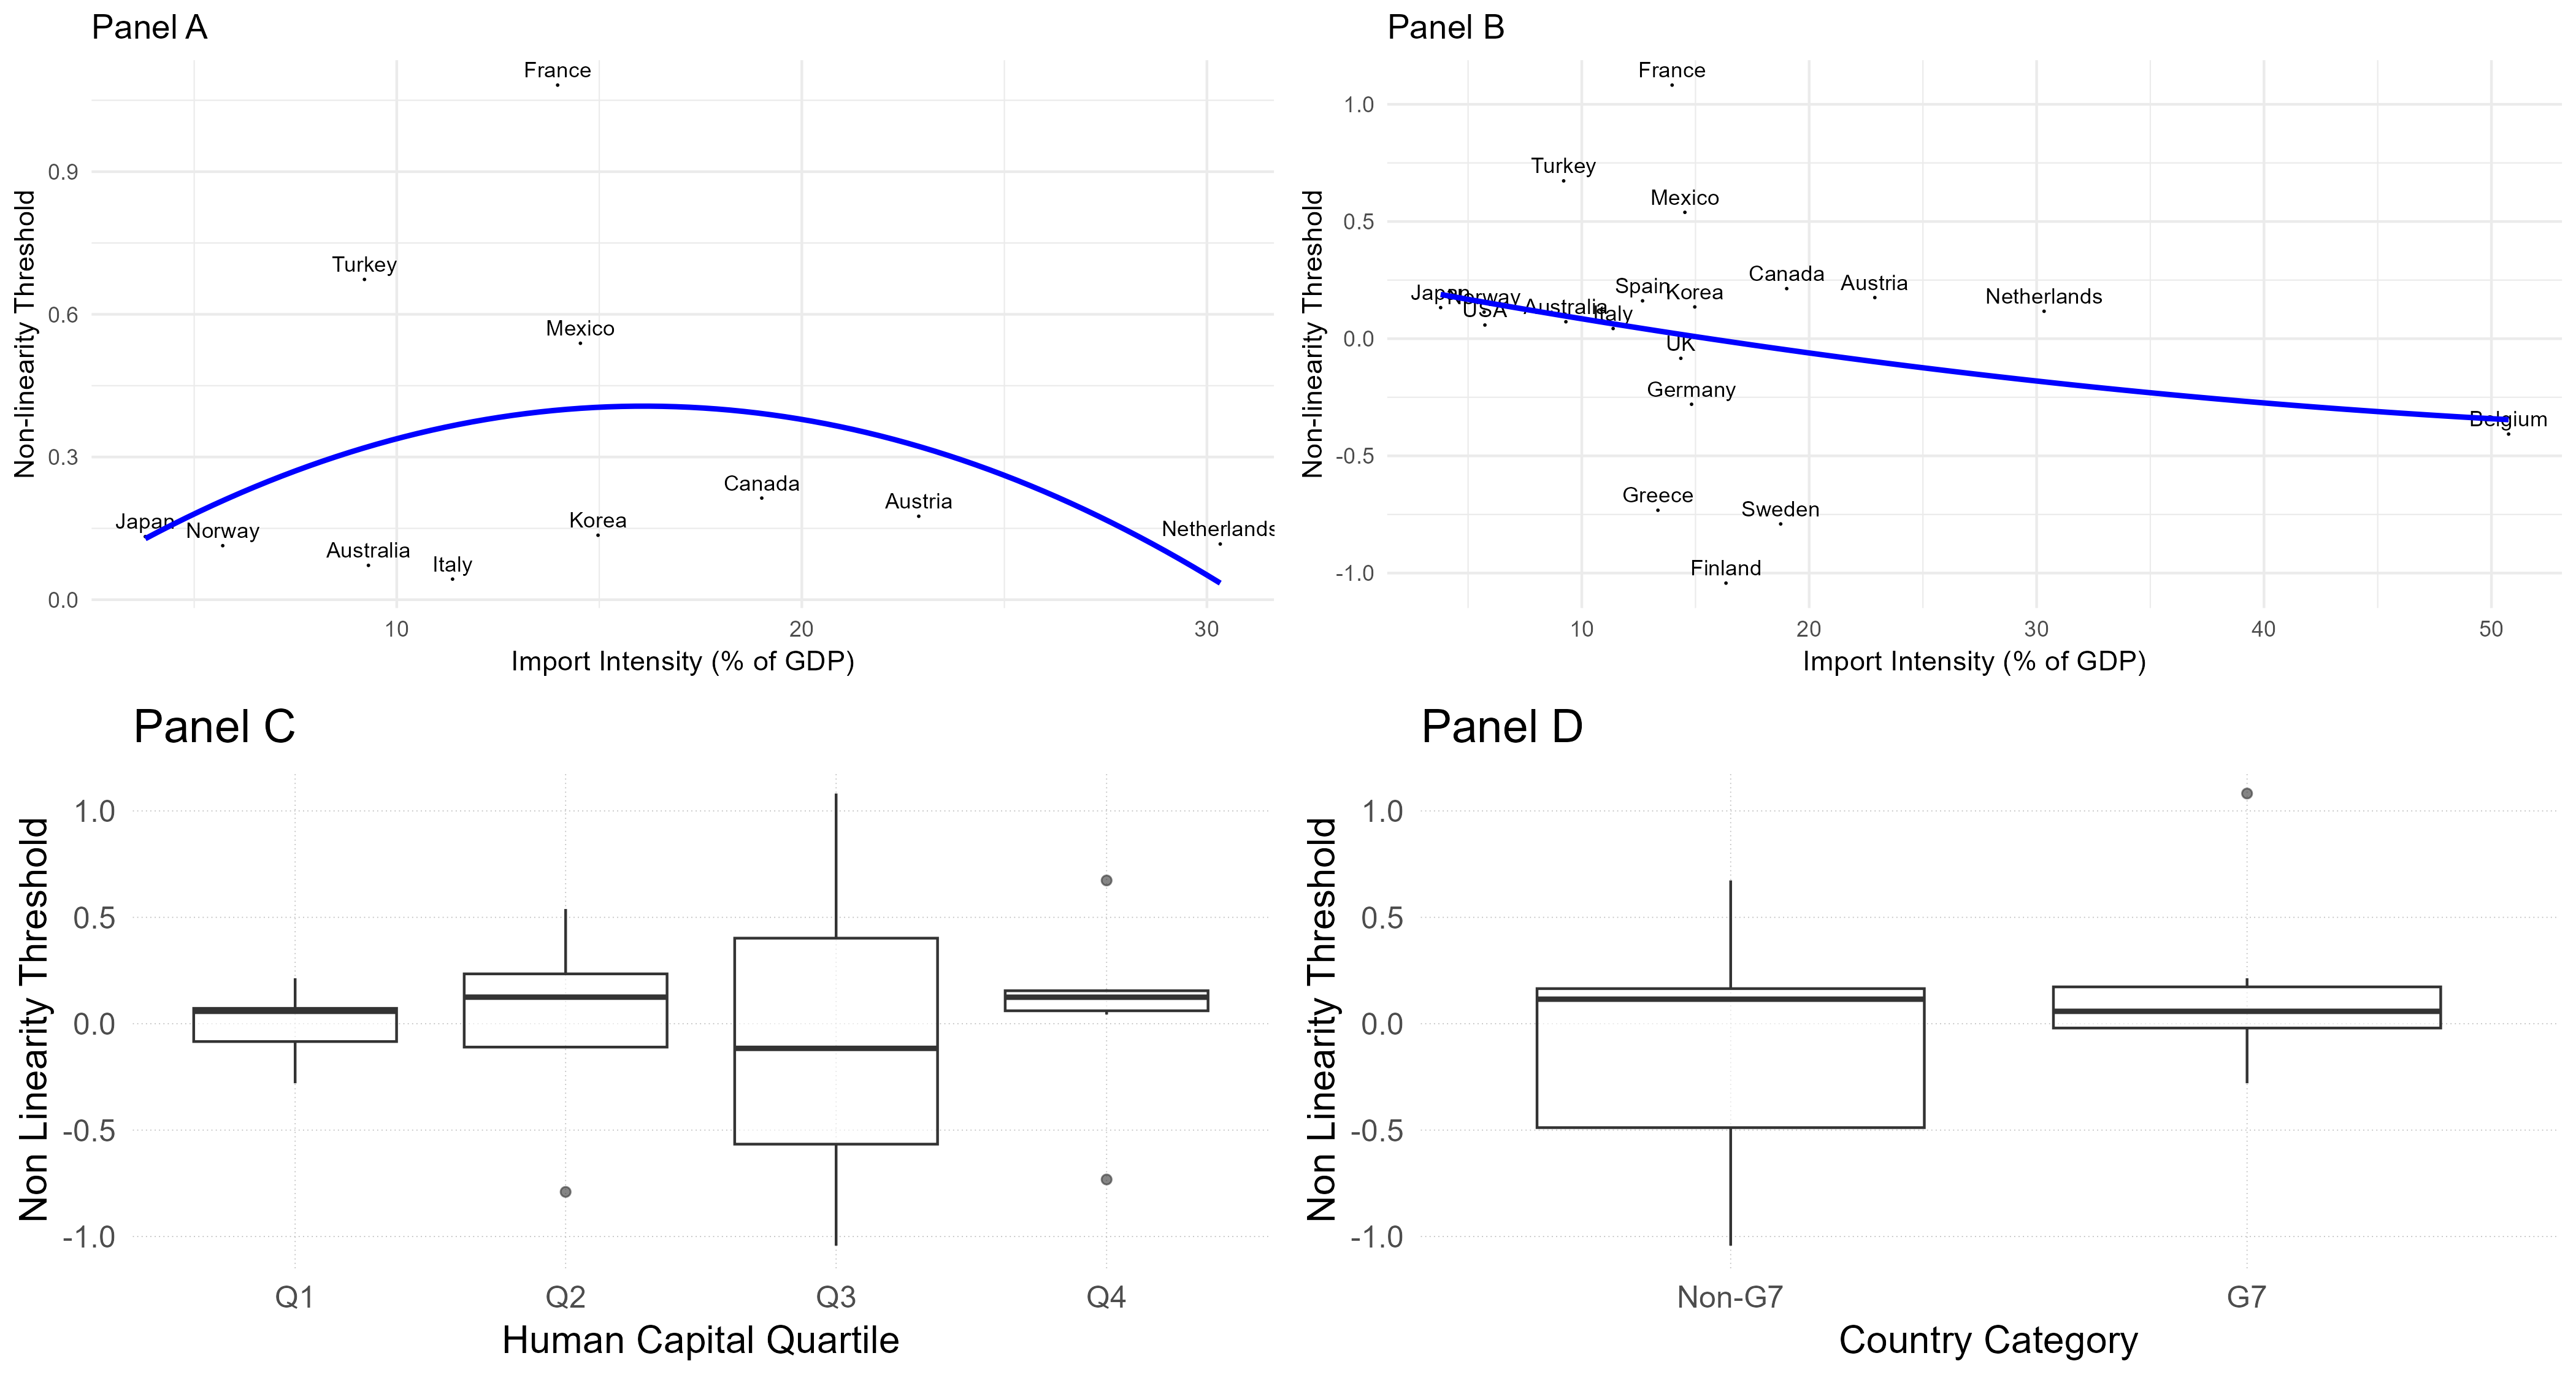
\includegraphics[width=1\linewidth]{NL.png}
    \label{fig: threshold}
    \justifying{\textit{Figure Notes: The above graphs plot the non-linearity threshold calculated as $\beta^f_i/\beta^{m*f}_i$ $\forall$ $i$. Panel A uses a sub-sample of countries that reveal an inverted U shaped relationship between $TFP$ and $S^f$. Panels B, C, and D use sub-samples excluding heavy outliers but including countries with thresholds below 0. They plot the non-linearity threshold against import intensity, human capital, and G7/Non-G7 countries.}}
\end{figure}

Panels B, C, and D use a sample of countries that exclude countries whose non-linearity thresholds are significant outliers, and attempts to understand heterogeneity in the thresholds by classifying countries into categories based on their import intensity, their human capital index, and their status as a G7 or non-G7 country. In Panel B, the threshold value decreases as average import intensity increases, suggesting that as import intensity rises, the turning point beyond which spillovers decrease becomes smaller, because markets becomes more saturated with foreign goods and services, leading to diminishing marginal returns from further imports. This market saturation means that the positive spillovers from trade start to taper off at a lower threshold. Therefore, the turning point where additional imports provide fewer benefits occurs sooner, reducing the average threshold value as import intensity rises.

Intuitively, countries with a higher human capital index would have a higher absorptive capacity, and therefore, a higher threshold \citep{Kneller2006}, but these differences cannot be seen in the selected sample of countries. The vintage human capital effects \citep{Chari1991, Comin2004} explain this observation: OECD countries give greater emphasis to developing domestic technologies rather than learning from foreign technologies, since most of these countries can be categorised as developed nations \citep{Coe1995}. There also does not appear to be any heterogeneity in the thresholds based on the countries' categorisation into G7 and non-G7 nations, which reinforces the previous finding that OECD countries, consisting of mainly developed nations, do not face much heterogeneity based on their sizes. 

\begin{table}[ht!]
\caption{Country-specific coefficients and thresholds}
\centering
\doublespacing
\setlength{\tabcolsep}{0.8pt}
\begin{tabular*}{\textwidth}{@{\extracolsep{\fill}} l c c c c c c c}
    \hline
 & $\beta^f$ & $\beta^{mf}$ & $-\beta^f/\beta^{mf}$ &  & $\beta^f$ & $\beta^{mf}$ & $-\beta^f/\beta^{mf}$ \\
\hline
AUS   & 0.129  & -1.782  & 0.072   & KOR     & 0.042  & -0.309  & 0.136  \\
AUT     & 0.010  & -0.058  & 0.175   & MEX     & 0.141  & -0.262  & 0.539  \\
BEL     & -0.042 & -0.104  & -0.407  & NED     & 0.054  & -0.464  & 0.117  \\
CAN     & 0.016  & -0.075  & 0.214   & NZL     & 0.161  & 0.039   & -4.102 \\
DEN     & 0.129  & 0.030   & -4.261  & NOR     & 0.082  & -0.718  & 0.114  \\
FIN     & 0.148  & 0.141   & -1.043  & POR     & 0.255  & 0.034   & -7.491 \\
FRA     & 0.055  & -0.051  & 1.082   & ESP     & -0.133 & 0.820   & 0.162  \\
GER     & 0.065  & 0.231   & -0.280  & SWE     & 0.193  & 0.245   & -0.790 \\
GRE     & 0.256  & 0.349   & -0.732  & TUR     & 0.095  & -0.141  & 0.673  \\
IRL     & -0.061 & -0.018  & -3.435  & UK      & 0.086  & 1.024   & -0.084 \\
ITA     & 0.013  & -0.298  & 0.043   & USA     & -0.050 & 0.856   & 0.058  \\
JPN     & 0.086  & -0.645  & 0.133   &         &        &         &        \\
\hline
\end{tabular*}
\label{tab:coefficients}
\justifying{\textit{Table Notes: Country specific coefficients presented from Model (2) in Table \ref{tab: nl}. $\beta^f$ represents the coefficient for foreign R\&D stocks, $\beta^{mf}$ represents the coefficient of the interaction of foreign R\&D stocks with $m$, and $-\beta^f/\beta^{mf}$ is the non-linearity threshold.}}
\end{table}

Table \ref{tab:coefficients} shows that some countries (e.g., Denmark, Finland, Germany, Greece, New Zealand, Portugal, United Kingdom) benefit from positive spillovers amplified by higher import shares, which is in line with the hypothesis of \citet{Lichtenberg1998} that countries experience higher spillovers with greater import intensities. There are also countries that have a negative coefficient for $S^f$ but positive coefficient for $m*S^f$ (Spain, United States), leading to a positive threshold but a U-shaped relationship. This pattern is consistent with \citet{Acharya2008}, who argue that, while import liberalization can reduce domestic productivity by increasing competition from foreign firms, it can also foster technological learning when imports are high in technology. In contrast, Belgium and Ireland have negative returns to productivity, which is worsened by increasing imports, which may be because of low quality imports when compared to Spain and the US. These findings imply that the relationship between foreign R\&D spillovers and productivity is dependent on trade patterns and trade intensity with countries having better technologies, as outlined by \citet{Fracasso2015}. 

Hence, it can be concluded that the threshold of non-linearities are heterogeneous across countries. Most countries in the sample have an inverted U-shaped relationship as earlier hypothesised, heterogeneity in which is determined by their import intensity. There are also countries which show an exponential relationship, that is, the direction of spillovers are intensified with greater imports. Countries may also show a U-shaped relationship, which may be because of country specific institutional factors \citep{Coe2009}, trade patterns \citep{Fracasso2015}, and their respective absorptive capacities \citep{Kneller2006}.  

\section{Conclusion}

This study investigates the presence of international R\&D spillovers sparked by the work of \citet{Coe1995} and makes two contributions to the existing literature on the subject. First, it updates the time-period taken by \citet{Coe2009} by taking a time-period of 49 years and a cross-section of 23 OECD countries and uses techniques which capture unobserved common shocks. Using the dynamic CCE estimator, this study reports statistically insignificant long-run coefficients for foreign R\&D stocks, but significant positive coefficient for domestic R\&D stocks, especially for G7 countries. It leads one to question the validity of the conclusions drawn by previous studies, and highlights that spillover effects turn insignificant when the econometric specifications accommodate unobserved common shocks and spillovers. Furthermore, the study examines heterogeneity in spillover coefficients across three key factors—G7/non-G7 status, human capital levels, and import intensity—revealing that G7 countries and countries in the top quartile of human capital index experience higher returns on domestic R\&D, while foreign R\&D returns diminish with rising import intensity.

The second contribution of this study lies in disentangling international knowledge spillovers by understanding non-linearities arising due to import intensity. The results suggest that there is a significant non-linear relationship for foreign R\&D in countries with an average import intensity of less than 15\%. However, there does not appear to be any heterogeneity in the threshold of such non-linearities based on human capital and G7/non-G7 countries.

In conclusion, this study attempts to improve the empirical rigour in the literature on international R\&D spillovers. Furthermore, it points towards non-linearities in R\&D spillovers, which existing literature has failed to recognise. The nature of spillover effects varies by country, so policies effective in one nation may be ineffective or harmful in another due to differing national contexts. Therefore, a limitation of this paper is that it ignores country-specific institutions which cause heterogeneity in spillovers.


\printbibliography[
heading=bibintoc,
title={References}
]

\appendix
\section*{Appendix}
\addcontentsline{toc}{section}{Appendices} 


\section{Unit Root Tests and Cointegration} \label{ap: A}

The cross-sectional Im-Pesaran-Shin (CIPS) test for unit root provided by \citet{Pesaran2007}, which augments the unit root test given by \citet{Im2003}, is used. It tests the null hypothesis that all panels follow a unit root process against the alternate of some panels being stationary. 

\begin{table}[h!]
\caption{Results of CD and CIPS Tests} 
\doublespacing
\setstretch{1.60}
    \centering
    \begin{tabular*}{\textwidth}{@{\extracolsep{\fill}} l c c c}
        \hline
        Variable & CD & \multicolumn{2}{c}{CIPS} \\
        \hline
        & & Without Trend & With Trend \\
        \cline{3-4}
        $TFP$ & 48.79*** & -1.240 & 0.865 \\
        $S^d$ & 110.49*** & -2.113** & 0.805 \\
        $S^{f:lp}$ & 110.34*** & -2.112** & 0.510 \\
        $m$ & 41.53*** & -0.905 & -0.473 \\
        $m*S^{f:lp}$ & 75.16*** & -1.595* & -1.494* \\
        $H$ & 107.63*** & -0.460 & -1.919** \\
        \hline
    \end{tabular*}
    \justifying
    \textit{The table presents the unit-root properties of the variables and results for cross-sectional dependence. *, **, and *** represent statistical significance at the 10\%, 5\%, and 1\% levels respectively.}
    \label{table: CIPS}
\end{table}

\begin{table}[ht!]
    \caption{Westerlund Cointegration Test Results}
    \doublespacing
    \centering
     \setlength{\tabcolsep}{2pt} % Adjust the separation between columns
    \begin{tabular*}{\linewidth}{@{\extracolsep{\fill}} lcccc}
        \hline
        Model & $G_t$ & $G_a$ & $P_t$ & $P_a$ \\
        \hline
        $TFP, S^d, S^{f:lp}$ & -2.404*** & -7.986** & -9.095*** & -5.158*** \\
        $TFP, S^d, mS^{f:lp}$ & -2.205*** & -7.928** & -9.915** & -5.980*** \\
        $TFP, S^d, S^{f:lp}, H$ & -2.706*** & -4.192 & -6.563 & -3.490 \\
        $TFP, S^d, mS^{f:lp}, H$ & -3.108*** & -4.211 & -8.980** & -3.753 \\
        \hline
    \end{tabular*}
    \justifying
    \textit{Table Notes: *, **, and *** represent statistical significance at the 10\%, 5\%, and 1\% levels respectively.}
    \label{table: cointegration}
\end{table}

Most variables appear non-stationary and cross-sectionally dependent; hence, checking cointegration is necessary for a DOLS model. To account for cross-sectional dependency, the \citet{Westerlund2007} panel cointegration test is used in Table \ref{table: cointegration}. The statistics presented in Table \ref{table: cointegration} show that the specifications tested are cointegrated.

\section{Robustness in Specification of Unobserved Process} \label{ap: C} 

Table \ref{tab: pooled} presents an error correction representation of the baseline specification using pooled OLS (POLS), two-way fixed effects (2FE), pooled common correlated effects (CCEP), mean group (MG), and common correlated effects mean group (CCEMG) estimators. The POLS and 2FE models assume homogeneous coefficients across countries; the latter considers country and time fixed-effects to capture unobserved heterogeneity. The CCEP model uses cross-sectional averages to account for unobserved common shocks, but does not impose heterogeneous coefficients. The MG model assumes heterogeneous coefficients but does not account for cross-sectional dependency. Finally, the CCEMG model uses contemporaneous cross-sectional average terms as regressors. 

\begin{table}[h!]
    \centering
    \doublespacing
      \setlength{\tabcolsep}{1pt} 
        \caption{Linear Dynamic Models (ECM)}
  \begin{tabular*}{\textwidth}{@{\extracolsep{\fill}}l*{5}{c}}
    \hline
        Variables & POLS  & 2FE & CCEP & MG & CCEMG  \\
         \hline
        $S^d$ & 0.042* & 0.070  & 0.111***  & 0.174** & 0.019 \\
         & (1.79)  & (1.16) & (3.37) & (2.22) & (1.24) \\
        $S^f$ & 0.001 & 0.008 & -0.022 & -0.076** & 0.022 \\
         & (0.09) & (0.007) & (-0.77) & (-2.04) &  (1.31) \\
        $ECT_{t-1}$ & -0.044*** & -0.029*** & -0.207*** & -0.209***  & -0.382*** \\
         & (-7.66) & (-3.48) & (-8.79) & (-7.41)  &  (-8.57) \\
         \hline
         Observations& 1104 &  1104 & 1104 & 1104 & 1104 \\
         $CD$& 50.65 & 70.70 & 45.22 & 19.82  & 7.75 \\
         $RMSE$& 0.021 & 0.019 & 0.018  & 0.018 & 0.017 \\
         \hline
    \end{tabular*}
        \justifying{\textit{Table Notes: Standard errors reported in parantheses. Short run variables included in regressions but not reported.*, **, and *** represent statistical significance at the 10\%, 5\%, and 1\% level respectively.}}
    \label{tab: pooled}
\end{table}



The diagnostic tests highlight that the use of cross sectional averages considerably reduces residual cross-sectional dependence, as demonstrated by the decrease in the \citet{Pesaran2004} CD statistic from 70.70 in the 2FE model to 45.22 in the CCEP model, and from 19.82 in the MG model to 7.75 in the CCEMG model. Although the null hypothesis of cross-sectional independence still cannot be rejected in the CCEP or CCEMG models, the results are quite encouraging for modelling with further lagged cross-sectionally averaged regressors. 

\end{document}
